%KECReportFormat.tex
%%%%%%%%%%%%%%%%%%%%%%%%%%%%%%%%%%%%%%%%%%%%%%%%%%%%%%%%%%%%%%%%%%%%%%%%%%%
%DO NOT MAKE CHANGES IN THIS FILE

\documentclass[12pt, a4paper]{report}
\usepackage[left = 1.5in, right = 1in, top = 1in, bottom = 1in]{geometry}%for margin
\usepackage{amsfonts, amsmath, amssymb} %for mathematical equations
\usepackage{graphicx} %for images
\usepackage{times} %font Times New Roman Font
\usepackage{float} %required if you use H(strictly here) position for floats
\usepackage[skip = 8pt,tableposition=top, figureposition=bottom]{caption}%adjust spacing of captions and specify where captions are
\usepackage{hyperref} % for easy Navigation in document, also puts links in TOC, LOF, LOT...
\usepackage{setspace} %to change line spacing in some portion \singlespacing \onehalfspacing \doublespacing
\usepackage{acro} %for List of Abbrreviation and Symbol
\acsetup{first-style = short} % set to display only short form on the command \ac{}

%packages required for complex tables
\usepackage{bigstrut} 
\usepackage{multirow}

\renewcommand{\contentsname}{Table of Contents} %Change TOC Heading ... default is "Contents" 

\parindent 0pt	%removes the indent in paragraph
\setlength{\parskip}{18pt}	%for paragraph spacing
\renewcommand{\baselinestretch}{1.5}   %Line Spacing = 1.5 line-spaces

%to reduce spacing in sections
\usepackage{titlesec}
\titlespacing*{\section}{0pt}{0pt}{0pt} %left, top, bottom spacings
\titlespacing*{\subsection}{0pt}{0pt}{0pt}
\titlespacing*{\subsubsection}{0pt}{0pt}{0pt}
\titlespacing*{\paragraph}{0pt}{0pt}{0pt}
\titlespacing*{\subparagraph}{0pt}{0pt}{0pt}

%adjust fontsizes\ of sections
\titleformat*{\section}{\fontsize{14pt}{18pt}\bfseries}
\titleformat*{\subsection}{\fontsize{13pt}{18pt}\bfseries}
\titleformat*{\subsubsection}{\fontsize{12pt}{18pt}\bfseries}
\titleformat*{\paragraph}{\fontsize{12pt}{18pt}\bfseries}
\titleformat*{\subparagraph}{\fontsize{12pt}{18pt}\bfseries}

%to reduce separation between points in list
\usepackage{enumitem}
\setlist[enumerate]{nosep} % no separation between items in enumerate
\setlist[itemize]{nosep} % no separation between items in itemize
%use \vspace{-18pt} before list to reduce paragraph spacing between list and preceeding paragraph.

%Changes for Chapter Heading Spacing and formats for numbered chapters
\makeatletter
\def\@makechapterhead#1{%
  %\vspace*{50pt}%
  {  \MakeUppercase{\ifnum \c@secnumdepth >\m@ne
        \fontsize{16pt}{1}\bfseries \@chapapp \space \thechapter\vspace{5pt}\\
    \fi
    \interlinepenalty\@M
     \bfseries #1}\par\nobreak
    %\vskip 0pt
  }}
\makeatother

%%%%%%%%%%%%%%%%%%%%%%%%%%%%%%%%%%%%%%%%%%%%%%%%%%%%%%%%%%%
%to adjust Heading spacings and fonts For unnumbered chapters, TOC, LOF ...
\makeatletter
% Redefine the \chapter* header macro to remove vertical space
\def\@makeschapterhead#1{%
  %\vspace*{50\p@}% Remove the vertical space
  {\newpage \parindent \z@ \raggedright
    \normalfont
    \interlinepenalty\@M
    \center \fontsize{16pt}{1} \bfseries \MakeUppercase{#1}\par\nobreak
    %\vskip 18\p@ % adjust space after heading 18pt
  }}
\makeatother 
%%%%%%%%%%%%%%%%%%%%%%%%%%%%%%%%%%%%%%%%%%%%%%%%%%%%%%%%%%%

%%%%%%%%%%%%%%%%%%%%%%%%%%%%%%%%%%%%%%%%%%%%%%%%%%%%%%%%%%%%%%%%%%%%%%%%%%%
% newcommand for generating Cover Page
\newcommand{\KECcoverpage}
{
\begin{titlepage}
\begin{center}
\Large{\textbf{KANTIPUR ENGINEERING COLLEGE}}\\
\large{\textbf{(Affiliated to Tribhuvan University)}}\\
\large{\textbf{Dhapakhel, Lalitpur}}\\
\vfill	%vertically fill the space 
\begin{figure}[h] % h: put logo "here"
\begin{center}

\includegraphics[width=25mm, height = 25mm]{images/logo.png}
\end{center}
\end{figure}

\large{\textbf{[Subject Code: \subCode]}}\\ %Change This Line
\large{\textbf{A \MakeUppercase{\project} \MakeUppercase{\doc} ON}}\\ %Change This Line
\Large{\textbf{\MakeUppercase{\projectTitle}}}\\

\vfill	%vertically fill the space 
\large{\textbf{Submitted by:}}\\
\large{\textbf{\submittedBy}}\\
\vfill	%vertically fill the space 
\textbf{A \MakeUppercase{\project} SUBMITTED IN PARTIAL FULFILLMENT OF THE REQUIREMENT FOR THE DEGREE OF \MakeUppercase{\degree}}\\

\vfill	%vertically fill the space 
\large{\textbf{Submitted to:}}\\
\large{\textbf{\submittedTo}}\\
\vfill
\large{\textbf{\defMonth, \defYear}}
\pagebreak
\end{center}
\end{titlepage}
}
%%%%%%%%%%%%%%%%%%%%%%%%%%%%%%%%%%%%%%%%%%%%%%%%%%%%%%%%%%%%%%%%%%%%%%%
% newcommand for generating Cover Page
%Title Page
\newcommand{\KECtitlepage}
{
\begin{titlepage}
\begin{center}
\Large{\textbf{\MakeUppercase{\projectTitle}}}\\

\vfill	%vertically fill the space 

\large{\textbf{Submitted by:}}\\
\large{\textbf{\submittedBy}}\\


\ifhassupervisor % Displays Supervisor name only if \hassupervisortrue
	\vfill	%vertically fill the space 
	\large{\textbf{Supervised by:}}\\
	\large{\textbf{\supervisor}}\\
	\large{\textbf{\degSup}}\\
\fi

\vfill	%vertically fill the space 
\textbf{A \MakeUppercase{\project} SUBMITTED IN PARTIAL FULFILLMENT OF THE REQUIREMENT FOR THE DEGREE OF \MakeUppercase{\degree}}\\

\vfill	%vertically fill the space 
\large{\textbf{Submitted to:}}\\
\large{\textbf{\submittedTo}}\\
\large{\textbf{Kantipur Engineering College}}\\
\large{\textbf{Dhapakhel, Lalitpur}}\\

\vfill
\large{\textbf{\defMonth, \defYear}}
\thispagestyle{empty}\\ %to remove page number
\pagebreak
\end{center}
\end{titlepage}
}
%%%%%%%%%%%%%%%%%%%%%%%%%%%%%%%%%%%%%%%%%%%%%%%%%%%%%%%%%%%%%%%%%%%%%%
%command for copyright page
\newcommand{\KECcopyright}
{
\chapter*{Copyright}%Required only for Final Defense of Major Project
\addcontentsline{toc}{chapter}{Copyright}
The author has agreed that the library, Kantipur Engineering Collage, may make this report freely available for inspection. Moreover the author has agreed that permission for extensive copying of this report for scholarly purpose may be granted by the supervisor(s), who supervised the project work recorded herein or, in their absence, by the Head of the Department wherein this project was done. It is understood that due recognition will be given to the author of this report and to the \submittedTo, Kantipur Engineering College in any use of the material of this report. Copying or publication or other use of this report for financial gain without approval of the \submittedTo, Kantipur Engineering College and author’s written permission is prohibited.\par Request for permission to copy or to make any other use of the material in this report in whole or in part should be addressed to:

Head\\
\submittedTo\\
Kantipur Engineering College\\
Dhapakhel, Lalitpur\\
Nepal
}
%%%%%%%%%%%%%%%%%%%%%%%%%%%%%%%%%%%%%%%%%%%%%%%%%%%%%%%%%%%%%%%%%%%%%%
%command for Approval Letter
\newcommand{\KECapproval}
{
\chapter*{Kantipur Engineering College
\vskip -10pt}%Required only for Final Defense of Major Project
\begin{center}
\fontsize{12.8pt}{1} %size decreaced to adjust department name in single line
\textbf{
\MakeUppercase{\submittedTo}\\ %for department name
}
\vskip 10pt
\fontsize{16pt}{1}
\textbf{APPROVAL LETTER}
\end{center}
\vskip -16pt
\addcontentsline{toc}{chapter}{Approval Letter}%
The undersigned certify that they have read and recommended to the Institute of Engineering for acceptance, a project report entitled "\projectTitle " submitted by \\
\submittedBy \\
in partial fulfillment for the degree of \degree. \par
{\vspace{25pt}
..........................................\\
Supervisor\\
\supervisor \\
\degSup\\
\vspace{25pt}\\
..........................................\\
External Examiner\\
\external\\
\degExternal\\
\vspace{25pt}\\
..........................................\\
\hod\\
Head of Department\\
\submittedTo
\vspace{10pt}\\
Date: \defMonth\space\defDay ,\space \defYear
\singlespacing\par
} %single spacing for the texts inside {}
}

%command for list of abbreviations
\newcommand{\KECloa}
{
\chapter*{List of Abbreviations}
\addcontentsline{toc}{chapter}{List of Abbreviations}
\vskip -42pt % to reduce space due to invisivle acronym class name
{
\singlespacing
\printacronyms[include-classes=abbr, name= ]
}

}

%command for list of symbols
\newcommand{\KEClos}
{
\chapter*{List of Symbols}
\addcontentsline{toc}{chapter}{List of Symbols}
\vskip -42pt % to reduce space due to invisivle acronym class name{
{
\singlespacing
\printacronyms[include-classes=symbol, name= ]
}
}

%command to adjust toc, lof, lot spacing
\newcommand{\KECadjusttocspacings}
{
\parskip 0pt % to remove paragraph spacing in TOC, LOF ...
\renewcommand{\baselinestretch}{0.1} % to adjust line spacing in toc
\newcommand*{\noaddvspace}{\renewcommand*{\addvspace}[1]{}}
\addtocontents{lof}{\protect\noaddvspace} %remove extra vertical space in LOF
\addtocontents{lot}{\protect\noaddvspace} %remove extra vertical space in LOT
} %includes the file KecReportFormat.tex that include all necessary formattings
%\usepackage[first-style=long]{acro}
%%%%%%%%%%%%%%%%%%%%%%%%%%%%%%%%%%%%%%%%%%%%%%%%%%%%%%%%%%%%%%%%%%%%%%%%%%%
%Define Macros for Details of your Project
\newcommand{\project}{Minor Project } %Specify "Major Project" or "Minor Project"
\newcommand{\projectTitle}{IOE RESULT AND NOTICE VIEWER WEBSITE} %specify "Title" of Your Project
\newcommand{\doc}{Final Report} % specify the document you are preparing eg. "Proposal", "Mid-Term Report" or "Final Report"32
% Note that You have to sibmit "Final Report" for Pre-final defense as well.
\newcommand{\subCode}{CT654} %specify Subject of Your Project
\newcommand{\degree}{Bachelor in Computer Engineering} %specify your degree
\newcommand{\submittedBy}%Specify Names and Roll/Symbol Numbers of the Project Group Members
{
%Edit Member Names and Roll/Symbol No. and adjust width (\makebox[width]) if necessary 
\makebox[7cm]{Aayush Shrestha \hfill [2882]}\\
\makebox[7cm]{Aliz Shrestha \hfill [28007]}\\
\makebox[7cm]{Ankit Kafle \hfill [28010]}\\
\makebox[7cm]{Kashyap Ghimire \hfill [28033]}
%\makebox[9cm]{Member Name \hfill [Roll/Symbol No.]}\\
} % Note that You must write your "Symbol Numbers"(Exam Roll Numbers) for Final Defenses

\newcommand{\submittedTo}{Department of Computer and Electronics Engineering} %specify your department
\newcommand{\hod}{Er. Rabindra Khati} %specify Head ot the department
\newcommand{\defYear}{2023} %Defense Year
\newcommand{\defMonth}{March} %Defense Month- January, February, ...
\newcommand{\defDay}{1} %specify Defense Day- 1, 2, ...

\newif\ifhassupervisor
\hassupervisorfalse % to display supervisor name use command- \hassupervisortrue
 
\newcommand{\supervisor}{Supervisor's Name} % Specify Name of Supervisor for Major Project
\newcommand{\degSup}{Supervisor's Designation\\Second Line of Designation (if required)} %Specify Designation of Supervisor for Major Project, use multiple lines (\\) if necessary
\newcommand{\external}{External's Name} %Specify Name of External for Major Project (Required for Black Book)
\newcommand{\degExternal}{External's Designation\\Second Line of Designation (if required)} %Specify Name of External for Major Project (Required for Black Book) , use multiple lines (\\) if necessary


%%%%%%%%%%%%%%%%%%%%%%%%%%%%%%%%%%%%%%%%%%%%%%%%%%%%%%%%%%%%%%%%%%%%%%%%%%%

%%%%%%%%%%%%%%%%%%%%%%%%%%%%%%%%%%%%%%%%%%%%%%%%%%%%%%%%%%%%%%%%%%%%%%%%%%%
%Define Abberviations and Symbols
% NOTE that Only those Abberviations and Symbols that are included in document(using command \ac{}) will be displayed in the List of Abberviations and Symbols.

%class 'abbr': for List of Abbreviations
\DeclareAcronym{OCR}{
    short = OCR,
    long = Optical Character Recognition,
    tag = abbr
}
\DeclareAcronym{LPR}{
    short = LPR,
    long = License Plate Recognition,
    tag = abbr
}
\DeclareAcronym{KNN}{ 
  short = KNN ,
  long  = K-Nearest Neighbor ,
  tag = abbr
}% declares acronym named "UN". Use \ac{UN} for short and \acl{UN} for long form. 

\DeclareAcronym{TTS}{
  short = TTS ,
  long  = Text To Speech ,
  tag = abbr
}
\DeclareAcronym{CNN}{
  short = CNN ,
  long  = Convolutional Neural Network ,
  tag = abbr
}
\DeclareAcronym{YOLO}{
    short=YOLO,
    long = You Only Look Once,
    tag= abbr,
}
\DeclareAcronym{LP}{
    short = LP,
    long = License Plate,
   	tag = abbr,
    }
\DeclareAcronym{GPU}{
    short = GPU,
    long = Graphics Processing Unit,
    tag = abbr
}
\DeclareAcronym{ANPR}{
    short = ANPR,
    long = Automatic Number Plate Recognition,
    tag = abbr
}
\DeclareAcronym{API}{
    short = API,
    long = Application Programming Interface,
    tag = abbr
}
\DeclareAcronym{BERT}{
    short = BERT,
    long = Bidirectional Encoder Representations from Transformers,
    tag = abbr
}
\DeclareAcronym{IAST}{
    short = IAST,
    long =  International Alphabet of Sanskrit Transliteration ,
    tag = abbr
}
\DeclareAcronym{UML}{
    short = UML,
    long =  Unified Modelling Language ,
    tag = abbr
}
\DeclareAcronym{ITRANS}{
    short = ITRANS,
    long = Indian Language Transliteration,
    tag = abbr
}
%%%%%%%%%%%%%%%%%%%%%%%%%%%%%%%%%%%%%%%%%%%%%%%%%%%%%%%%%%%%%%%%%
% class `symbol': for List of Symbols
\DeclareAcronym{transparencyFactor}{
  short = \ensuremath{\alpha} ,
  long  = Transparency Factor ,
  sort  = Transparency Factor , % string to compare for sorting symbols... default string is the acronym name -"transparencyFactor"
  tag = symbol
}% declares acronym named "transparencyFactor". Use \ac{UN} for short and \acl{UN} for long form.

\DeclareAcronym{areaOfTriangle}{
  short = \ensuremath{a} , % use \ensuremath{a} instead of $a$
  long  = Area of Triangle ,
  sort  = Area of Triangle , % string to compare for sorting symbols
  tag = symbol
}
%%%%%%%%%%%%%%%%%%%%%%%%%%%%%%%%%%%%%%%%%%%%%%%%%%%%%%%%%%%%%%%%%%%%%%%%%%%%%%%%%%%%%%%%%%%%%%%%%%%%

%%%%%%%%%%%%%%%%%%%%%%%%%%%%%%%%%%%%%%%%%%%%%%%%%%%%%%%%%%%%%%%%%%%%%%%%%%
%The Document
\begin{document}

\KECcoverpage % command defined in KECReportFormat
\KECtitlepage % command defined in KECReportFormat

\pagenumbering{roman} % starts pagenumberins in Roman numerals i, ii, ...
\addcontentsline{toc}{chapter}{Acknowledgement}
\chapter*{Acknowledgement}

Firstly, we would like to give our most profound appreciation towards our project manager, Er. Bishal Thapa for his steady direction, support and proposals amid the course of our project development. We are moreover profoundly obliged to Er. Sahaj Shakya for his important recommendations and insights on web scraping and OCR. We would also like to thank our class teacher Er. Nishan Khanal who helped us during the course of our project when we encountered some errors and glitches. Besides, we would like to thank the Department of Computer and Electronics of Kantipur Engineering College for giving us resources for the completion of the project. Moreover, we are exceptionally thankful to Er. Suman Shrestha and Mr. Tek Narayan Adhikari for helping us by providing additional resources in the form of college emails which were used during the course of project. At long last, we would like to recognize and thank everybody who helped us specifically or in a roundabout way in this extend.



 



\chapter*{Abstract} % The summary of your report
\addcontentsline{toc}{chapter}{Abstract}%to include this chapter in TOC 
In a real world scenario, such as a college campus, the information in the form of notice, 
hand-written manual, and verbal message, is being spread among the students. Today 
it is of the essence to not only use the predictable forms of statements, but also new 
forms such as cell phone technology and websites for faster and easier communication 
among the students. Viewing the results, notices immediately after the publication is a 
challenge for many students. due to which it consumes student’s time and resources. 
To overcome this, a website will be designed and developed that allows the students of 
Kantipur Engineering College to login with a unique ID that allows them to view 
results, notices and send out notification regarding if the registered students have passed 
the exam or not. We use the concept of Optical Character Recognition(OCR) to scan 
the symbol number of the students and check their result status and send the user result 
status directly to their emails. For extracting the notices from Institute of Engineering
(IOE), we use the algorithm of Web Scraping to fetch the important notices that are 
useful for the students.

\par
\textbf{\textit{Keywords$-$}}{\textit{Optical Character Recognition,}}{\textit{Web Scraping,}} 

\par
%to display members name under Acknowledgement
%\begin{flushright}
%\vskip -20pt
%\setstretch{1.2}
%\submittedBy
%\end{flushright}

%to adjust spacings for TOC, LOF, LOT
{
%%%%%%%%%%%%%%%%%%%%%%%%%%%%%%%%%%%%%%%%%%%%%%%%%%%%%%%%%%%%%%%%%%%%%%%%%%%
%TOC, LOF and LOT
\KECadjusttocspacings % defined in KECReportFormat.tex to adjust spacings
\makeatletter
% to add vskip of 18 point which is reduced when parskip is set to 0 in \LECadjustspacings
\def\@makeschapterhead#1{%
  %\vspace*{50\p@}% Remove the vertical space
  {\newpage \parindent \z@ \raggedright
    \normalfont
    \interlinepenalty\@M
    \center \fontsize{16pt}{1} \bfseries \MakeUppercase{#1}\par\nobreak
    \vskip 18\p@ % adjust space after heading 18pt
  }}
\makeatother 

\tableofcontents % prints table of contents
\listoffigures % prints list of figures
\addcontentsline{toc}{chapter}{List of figures}

%\addcontentsline{toc}{chapter}{Acknowledgement}

\chapter*{List of Abbreviations}
	CSS:  Cascading Style Sheet\\
	DFD: Data Flow Diagram\\
	EMAIL: Electronic Mail\\
	HTML: Hyper Text Markup Language\\
	IOE: Institute of Engineering\\
	KEC: Kantipur Engineering College\\
	OCR: Optical Character Recognition \\
	PHP: Hypertext Preprocessor\\
	SQL: Structured Query Language\\
	URL: Uniform Resource Locator\\
	VIPS:Vision Based Page Segmentation

\addcontentsline{toc}{chapter}{List of abbreviations}	
	
	
%\listoftables % prints list of table
}
%%%%%%%%%%%%%%%%%%%%%%%%%%%%%%%%%%%%%%%%%%%%%%%%%%%%%%%%%%%%%%%%%%%%%%%%%%%

%comment this chapter if you don't have List of Abbreviations
%\KECloa % defined in KECReportFormat

%comment this chapter if you don't have List of Symbols
%\KEClos % defined in KECReportFormat

\newpage
\pagenumbering{arabic} % starts pagenumbering in arabic numerals

\chapter{Introduction}
\section{Background}\label{sec:bkgrnd}%label your section if you require to refer them somewhere else in your document.
 With the advancement in time and technology, there is a need for faster dissemination 
of information. The increasing advantages of automated systems now are at their 
highest position thus many manual processes are automated. Since the automated 
system is demanded now-a-days, educational infrastructures like colleges needed their 
manual system to function on Mobile Computing Systems [1]. Today's world is the 
world of information and technology. Small and big tasks, meetings can be attended 
through different mobile website. Viewing a website frequently for notices is a hectic 
thing to do. Similarly verifying the results immediately after the publishment is also 
quite difficult as the result may come anytime and the particular user can be unaware 
about it.


So creating a user-friendly website that provides the user to view the important notices 
of IOE and providing notification every time a notice has been published is an ideal 
thing to do. The main goal of this project is helping the student to view the notices from 
IOE. Not only viewing the notices but also helping the students to view their result 
status immediately after the publishment is the main aim of the project. Not limited to 
a single stream, our website facilitates on different streams and every student of every 
field can gain access to our website which provides different facilities.


  
\section{Problem Statement}
In today's context, time is a key factor in everyone’s life. This statement is true for 
everyone including students. For a delicate topic like viewing exam results. The process 
should be quick as students are worried about their results. These processes are very 
time consuming and tedious. Most of the important notices are missed by the students 
because there is a lack of a proper notification system. So to solve these issues we have 
decided to develop the website in order to help the students to view their result status 
and be updated with the latest notices.

Furthermore, it is challenging to obtain manual records of the cars that utilized the parking lot in the future. The database built into our system can give historical records in an emergency or when a record is urgently needed to help with emergency control.


\section{Objectives}
\begin{enumerate}[label=\Roman*]
\item To implement easy result viewing for all the faculties. 
\item  To send the result status automatically via email to users after publishment.
\item To provide an effective notice display system
\end{enumerate}
	

   

\section{Application Scope}
The system being designed is economical with respect to the students’ point of view. 
The goal is to extract useful information from unstructured data using the concept of 
information retrieval, filtering and secure random algorithms. Our basic approach 
attempts to develop a website which can be used to make this process easier, secure and 
less error prone. This project provides a platform to extract real time data from IOE 
websites. It can be used as a tool to see the result status of the students according to 
their semester result.


\section{Features}
\begin{enumerate}
	\item  Provides an efficient and easy way to view notices.
	\item  Provides easy to use interface.
	\item Provides subscription based result viewer.
	\item  Provides quick access to view result status of students
\end{enumerate}
\section{Feasibility Study}
The feasibility study is one of the main important things to be considered for the project 
development. The feasibility study must be done for different factors affecting the 
project. Here are some factors whose feasibility study should be done for our project.
\subsection{Economic Feasibility}
Economic feasibility attempts to weigh costs of developing and implementing a new 
system, against the benefits that would accrue from having the new system in a place. 
This feasibility study gives the top management the economic justification for the new 
system. A simple economic analysis which gives the actual comparison of costs and 
benefits is much more meaningful meaning in this case. In addition, this proves to be a 
useful point of reference to compare actual costs as the project progresses. There could 
be various types of intangible benefits on account of automation. These could include 
increased customer satisfaction, improvement in product quality, better decision 
making, and timeliness of information, expediting activities, improved accuracy of 
operations, better documentation and record keeping, faster retrieval of information, 
better employee morale
\subsection{Technical Feasibility}
 Since the proposed system uses software technologies and tools which are freely 
available and technical skills required can be tricky but are manageable. There are many 
free machine learning libraries available for data analysis and predictions with proper 
documentation and courses. The hardware system in the project need not be highly 
computing but requires normal computing and the system server must be adequate and 
4
manageable in the future. so it is seen that the hardware and software meet the needs of 
the system. So it’s clear that the proposed project is technically feasible.
\subsection{Operational Feasibility}
Though the advancement in technologies, any kind of system software or application is 
no longer hard to operate. Thus the user needs to be only a bit familiar with the software 
system backed with graphical explanations and that can be easily understood faster in 
time with usage. This system highly focuses on design-dependent parameters like 
reliability, maintainability, supportability, usability, predictability, sustainability, 
affordability, etc. So, the project is feasible in operation.
\subsection{Schedule Feasibility}
Schedule Feasibility is defined as the probability of a project to be completed within its 
scheduled time limits, by a planned due date. If a project has a high probability to be 
completed on-time, then its schedule feasibility is appraised as high. Schedule 
feasibility ensures that a project can be completed before the technology becomes 
unnecessary. Since there are many features in our project but can be implemented in a 
quality way it has a very high probability to be completed on time.
\begin{figure}[h!]
    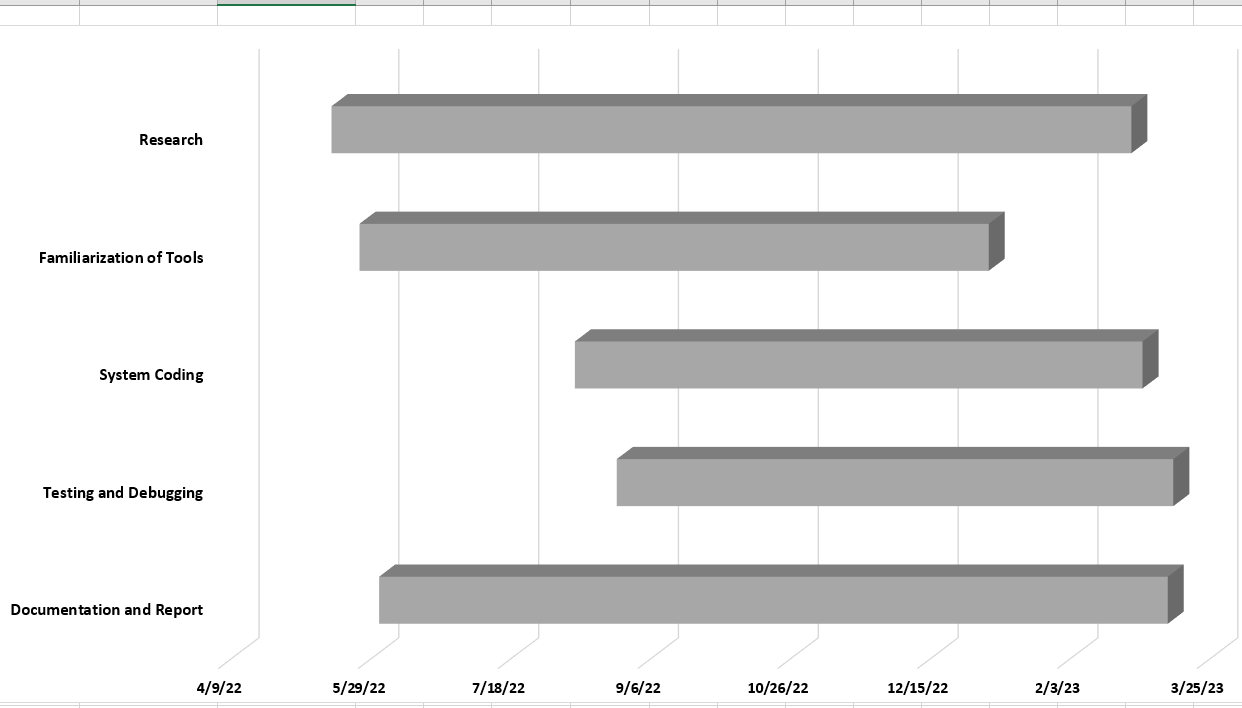
\includegraphics[scale=0.35]{images/Gantchart.png}
    \caption{Gantt Chart}
    \label{fig:my_label}
\end{figure}
\section{System Requirements}
The system requirements for the project are as follows:

\subsection{Development Requirements}
\subsubsection{Hardware Requirement(Minimum)}
\begin{itemize}
    \item  PC with a minimum specification of 8GB RAM and a sixth generation i5 
processor
\end{itemize}

\subsubsection{Software Requirement}

\begin{itemize}
    \item Microsoft Windows 7/8/10 (32 or 64 bit) or Mac OS

 
\end{itemize}

\subsection{Deployment Requirements}

\subsubsection{Hardware Requirement(Minimum)}
\begin{itemize}
    \item  More than 1.5 GHz clock speed 
    \item  Minimum 4GB RAM
\end{itemize}

\subsubsection{Software Requirement}
\begin{itemize}
    \item  Visual Studio Code
    \item  Pycharm
\end{itemize}


\chapter{Literature Review}
\section{Related Projects}

	\begin{itemize}
	
		\item IOE Syllabus : IOE Syllabus is a website in which students can see the notices, faculty syllabus, faculty 
notes, etc. Also students can get collection of past questions from this website.
			\item Onlineocr.net : A user friendly and free online OCR converter tool service to extract text from picture 
and that is available free of cost at the internet, help in doing Optical character 
recognition online.
		
\end{itemize}
\section{Related research}

In recent years, the use of technology and the popularity of e-commerce have led to a 
significant increase in the number of online shopping websites available. While this 
makes it convenient for people to shop online, it can also be time-consuming and 
require a lot of effort to search for the best deals and offers on these websites. In order 
to address this issue, the authors of the paper "Exploiting Filtering approach with Web 
Scraping for Smart Online Shopping" have developed a web scraping framework that 
allows users to efficiently gather product information and deals from multiple ecommerce websites. The framework is implemented using front-end technologies such 
as HTML (Hypertext Markup Language) and CSS (Cascading Style Sheet) as well as 
a back-end language, PHP (Hypertext Preprocessor). It uses Python libraries and 
HTML tags to write the scraping scripts, and the results are displayed dynamically to 
the user rather than being stored in a local database. According to the authors, this 
framework has a high accuracy rate of 93% and is efficient in terms of computation and 
time required. The goal of the framework is to make it easier for people to find the best 
deals and offers on e-commerce websites and save them time and effort in the process.[2] 
\\
\\
The paper "Barcode Character Defect Detection Method Based on Tesseract-OCR" 
aims to address the increasing quality requirements for barcodes as their use becomes 
more widespread with the advancement of information technology. However, during 
the printing process, various defects can occur, such as flying ink, missing print, wrong 
print, black spots, and improper registration, which can be caused by factors such as 
poor typography, inadequate printing equipment, and imperfect printing technology. 
The traditional method of manually sorting defective barcodes is inefficient and prone 
to error due to the influence of various factors, leading to low precision in detection. In 
order to address these issues, the authors propose a method for detecting defects in 
barcodes using Tesseract-OCR (Optical Character Recognition) software. This method 
involves segmenting the barcodes using horizontal projection, recognizing the 
characters in the barcodes using Tesseract-OCR, and applying the Levenshtein 
Distance algorithm to detect character defects. The authors conducted experiments 
using 1000 barcode images, and the results showed that the proposed method had an 
accuracy of 94.3% in detecting defects, indicating its feasibility as a method for 
detecting barcode defects.[3]
\\
\\
The paper “NewsOne — an aggregation system for news using web scraping method” 
is an online platform that aggregates and summarizes the latest news updates from 
multiple national and international sources. It presents this information in a concise and 
easy-to-read format, and is designed to allow users to quickly and easily access the 
news without wasting time searching or waiting for content to load. To achieve this, 
NewsOne employs web scraping and crawling techniques to extract news content from 
various websites, which it then categorizes based on user interest. The platform is also 
service-oriented, allowing users to interact with each other from across the web. 
NewsOne uses a bot that dynamically extracts content from the stored URL's RSS feeds 
at set intervals, which are added to a database by the platform's administrators or sub-administrators. This model of categorization is designed to extract useful information 
for classifying news articles into specific categories, such as Just-In, Technology, 
Health, Science, Sports, Business and Economics, and Entertainment. NewsOne's user 
experience is flexible, allowing readers to choose the categories of news that interest 
them and read the news for free and as quickly as possible. In addition, users have 
access to up-to-the-minute daily news coverage and headlines from over 100 fully 
licensed and trusted news sources from around the world. Finally, the platform also 
provides recommendations and thoughts for future development [4].





\chapter{METHODOLOGY}

\section{Working Mechanism}

\begin{figure}[h]
\centering
    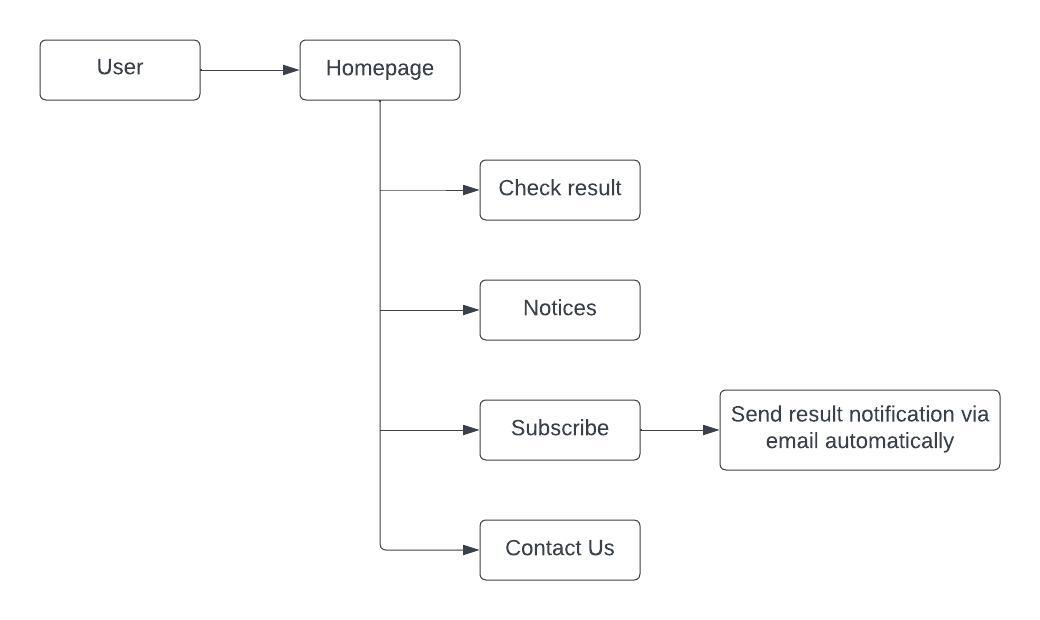
\includegraphics[scale=0.7]{images/block.jpg}
    \caption{Block diagram of the system}
    \label{fig:my_label}
\end{figure}
\begin{enumerate}
	\item Homepage: At first, the user interacts with the homepage of our system where they will be able to 
select options such as Check Result, Notices, Subscribe and Contact Us section.

	\item View Notices: One major feature of the website is to show Notices published by IOE. This feature 
now allows the user to view notices in real time after the IOE has published it. This 
feature can be implemented by the use of web scraping in which the website 
exam.ioe.edu.np will be scraped for notices. To view notices it is not necessary that the 
user must be subscribed.
	\item  View Results: Viewing results immediately after the publication with a proper interface is a hard thing 
to do. So with the webpage, the user can verify the result and see if they have passed 
the exams. To use this feature, the user doesn’t require to be subscribed in into the 
8
system. But to use the feature of getting automatically notified via email regarding the 
result status, the user must be subscribed using the email provided by KEC. The 
webpage admin automatically sends activation email to the subscriber and only after 
the subscription is activated, then after the publishment of result, the system 
automatically sends them an email regarding if they have passed or not. This can be 
achieved by using web scraping and OCR scan.
	\item  Subscribe: Viewing results immediately after the publication with a proper interface is a hard thing 
to do. So with the webpage, the user can verify the result and see if they have passed 
the exams. To use this feature, the user doesn’t require to be logged in into the system. 
But to use the feature of getting automatically notified via email regarding the result 
status, the user must be logged in using the email provided by KEC. The webpage 
automatically verifies the user and sends them an email regarding if they have passed 
or not. This can be achieved by using web scraping and OCR scan.
	\item  Contact Us:If any problem arises then the user can directly contact the developer to solve the issue.
The user must fill up the form where they have to insert their Name, Email, Subject and 
the message they want to send. The mail is now sent to the developers team email 
address
	
\end{enumerate}
\subsection*{ Web Scraping}
Web scraping is the process of collecting structured web data in an automated fashion. 
It’s also called web data extraction. Some of the main use cases of web scraping include 
price monitoring, price intelligence, news monitoring, lead generation, and market 
research among many others. In general, web data extraction is used by people and 
businesses who want to make use of the vast amount of publicly available web data to 
make smarter decisions. For our project we will use web scraping to extract the IOE 
notices and result from their website [5].
\begin{itemize}
	\item Cropping the image: First , the image after the detection of the position of the license plate and the bounding box formulation is cropped according to the coordinates of the bounding ox so that we are resulted with  the number plate from where the character extraction is to be done.
	\item Noise reduction and gray scaling: In order to male the image suitable for the character recognition, the image is filtered for the removal of noise and followed by the gray scaling of the cropped image so that the characters which are to be detected are separated from the background color. The conversion of image into black and white that is, improving the contrast causes better performance of the model.
\end{itemize}
The processed image is then sent through the process of OCR where the characters that are present in the image are extracted . The extraction process or the character recognition process is done with the help of either pattern recognition or feature recognition.
\section*{Procedure for Web Scraping}
\begin{enumerate}
\item Start
\item Create scraping template
\item Browse website
\item If the content is found, go to step 5, else repeat step 3
\item Get the link post
\item Explore the link post
\item Get the required data (Data extracted)
\item Stop
\end{enumerate}
\newpage
\section*{Flowchart of Web Scraping}
\begin{figure}[h]
\centering
    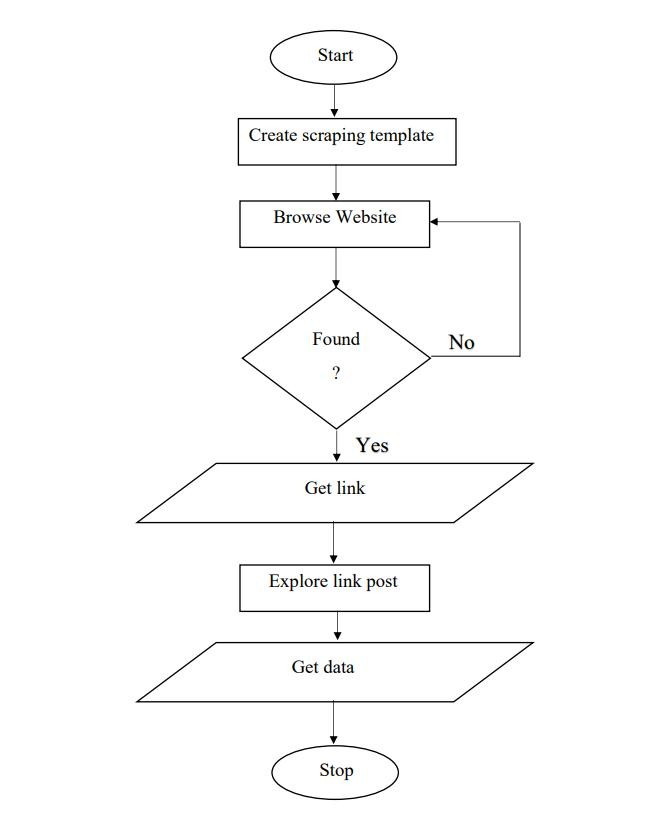
\includegraphics[scale=0.7]{images/vips.jpg}
    \caption{Flow Chart of Web Scraping}
    \label{fig:my_label}
\end{figure}
\section*{VIPS BASED SEARCHING}
\begin{enumerate}
\item Start
\item Construct parse tree for the HTML tags
\item Isolate all the anchor tags
\item Search for the result and notices inside the anchor tag
\item If result and notices are present, go to step 6, else go to step 7
\item Extract the content of anchor tag
\item If the entire webpage is scraped, go to step 8, else go to step 4
\item Stop
\end{enumerate}

\section*{Flowchart based on VIPS}
\begin{figure}[h]
\centering
    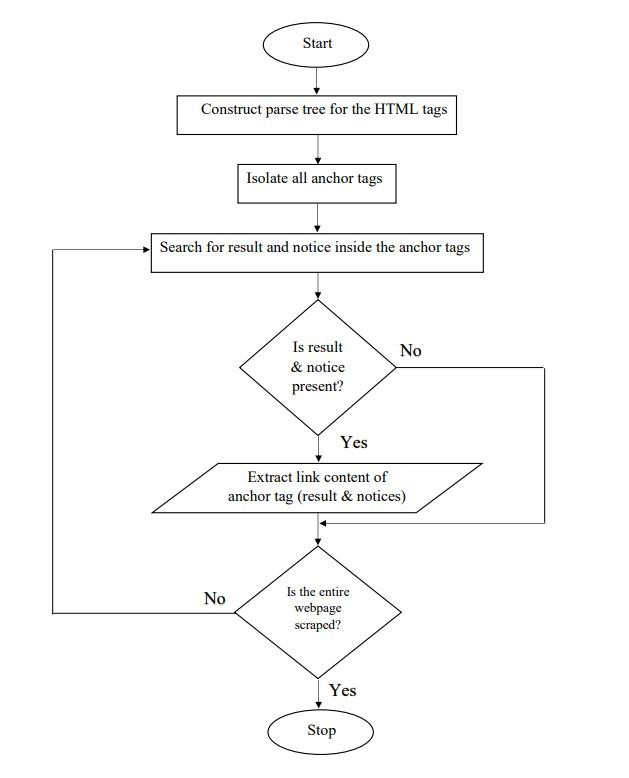
\includegraphics[scale=0.7]{images/vips1.jpg}
    \caption{Flowchart based on VIPS}
    \label{fig:my_label}
\end{figure}
\section*{Implementation of Web Scraping}
\begin{enumerate}
\item At first, the website of IOE is visited. After this, the site is explored.
\item The HTML content of the link is explored up until 10 pages initially to gather data into the database.
\item Now the entire webpage is converted into a parse tree through the use of an HTML parser. As from the inspection of the webpage, we found that the data of the notices and results along with the date of publishment and the link of the PDF file for the notices and results were stored by forming a table. The publishing date of the results and notices were stored in the third data cell for every table row. Also, every table row was considered for the extraction of the PDF file and the title for the notice and result. Only the notices and results of BE were taken in this stage.
\item Following the above step, the entire table rows of the table were explored and the title of the notices and results, which were present in the content of the \verb|<span>| tag, was extracted. Also, the link for the PDF was present in the \verb|<href>| part of the anchor tag, which was also extracted.
\item On observation of the actual PDF link for the notices and results, we encountered a problem in which the \verb|%20| part of the link was regarded as space which caused the actual link of the PDF to break. This was easily solved by replacing the space with \verb|%20| and joining the starting of the URL \verb|"https://exam.ioe.edu.np"| with the link from the \verb|<href>| tag.
\item Now the filtered title obtained from the content of \verb|<span>| from step 4, the date of the PDF obtained from step 3, along with the link of the PDF file obtained at the end of step 5, was inserted into the built-in SQLite database with a constraint that if the link of the notices and results were already present in the top of the database, then the insertion process would stop.
\end{enumerate}
\subsection*{Optical Character Recognition(OCR)}
OCR also referred as text scan is the process that extracts and repurposes data from 
scanned documents, camera images and image-only pdfs. OCR systems use a 
combination of hardware and software to convert physical, printed documents into 
machine-readable text. For our project we will use OCR to extract the symbol number 
as a string and then we will compare the symbol number that has been obtained with 
the help of OCR scan to the symbol number of the students. If the symbol number 
12
matches, then the backend of our project will send an email to the registered users 
automatically and then the students can know whether they have passed or not.

In our project the OCR scanning will be performed using a library in python.
\section*{Implementation Of OCR}
\begin{enumerate}
\item First, extract the PDF file's link from the database.
\item Using the link from step 1, extract the PDF file.
\item Convert the extracted PDF to an image format.
\item Scan the characters from the image and save the resulting string in the database.
\end{enumerate}



\newpage
\section{\ac{UML} Diagrams}
\subsection*{Use Case Diagram}
\begin{figure}[h!]
    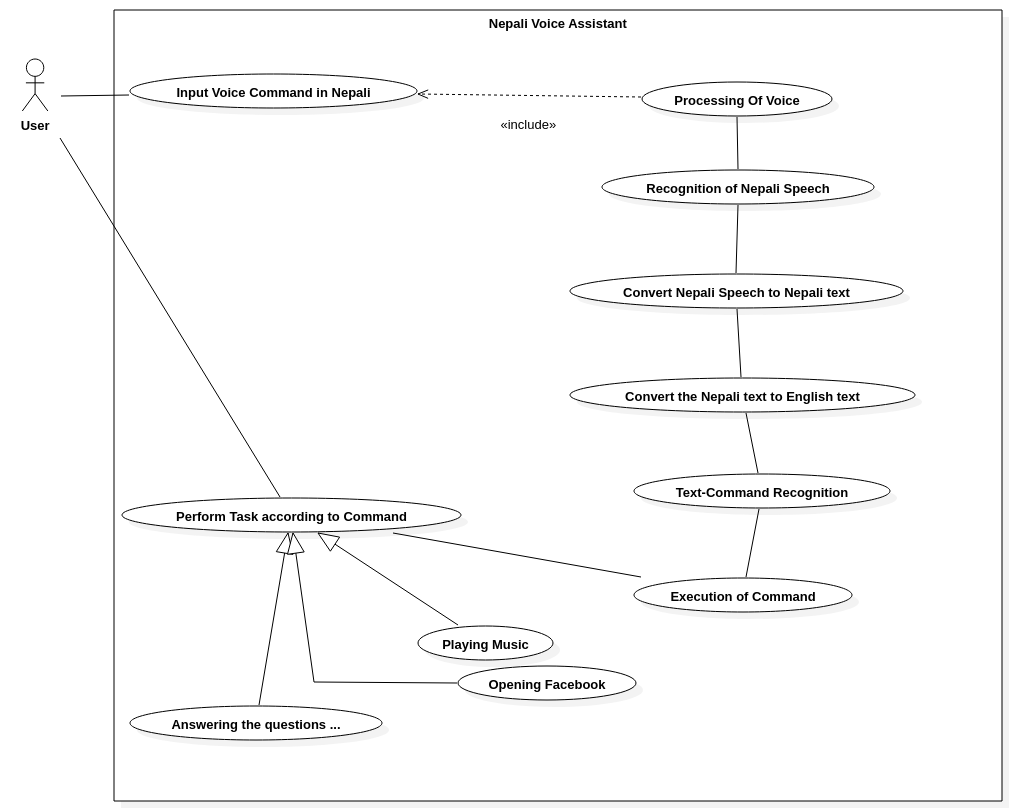
\includegraphics[scale=0.45]{images/usecase.png}
    \caption{Use Case Model of the System}
    \label{fig:my_label}
\end{figure}
\newpage
\subsection*{DFD Diagrams}
\begin{figure}[h]
    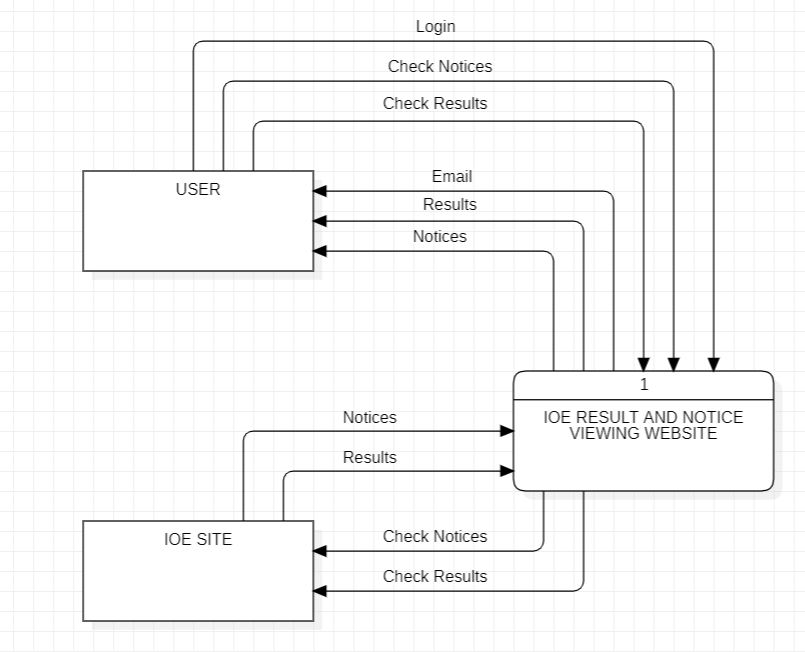
\includegraphics[scale=0.5]{images/dfd0.png}
    \caption{DFD Level 0 of the System}
    \label{fig:my_label}
\end{figure}
\newpage
\begin{figure}[tbh]
    \centering
    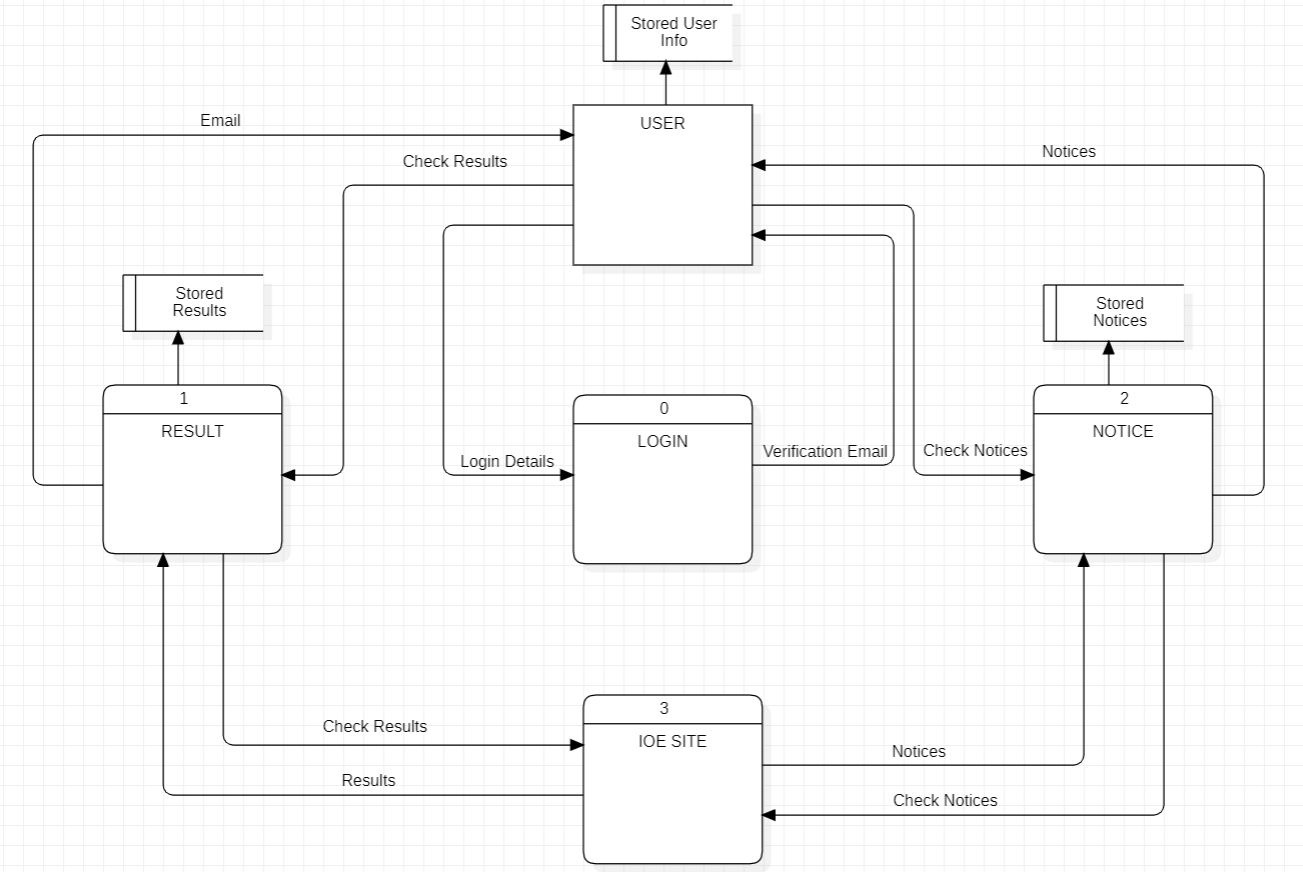
\includegraphics[scale=0.35]{images/DFD LEVEL1.png}
    \caption{DFD Level 1 of the system}
    \label{fig:my_label}
\end{figure}

\section{Software Development Model}
The incremental model is one of the easiest to implement software development life 
cycle models. There are certain scenarios where the initial or the core software 
requirements are clearly defined, but the actual span or the full set of features of the 
project are unknown. Moreover, the development company might decide to not give 
the full functionality of the software in one go. Rather they prefer to give it out through 
periodic updates. Or the client requests some functionality enhancements during the 
process of development. In such cases, the incremental model is used.
\\
\\
In the first phase we performed Web Scraping and extracted all the results and notices 
from the website. In the second phase we used Database using MYSQL and inserted all 
the notices and results in the database. In the third phase we implemented the concept 
of OCR. In the fourth phase we performed mailing methods to send the email of result 
status to the subscribed students
\begin{figure}[h]
    \centering
    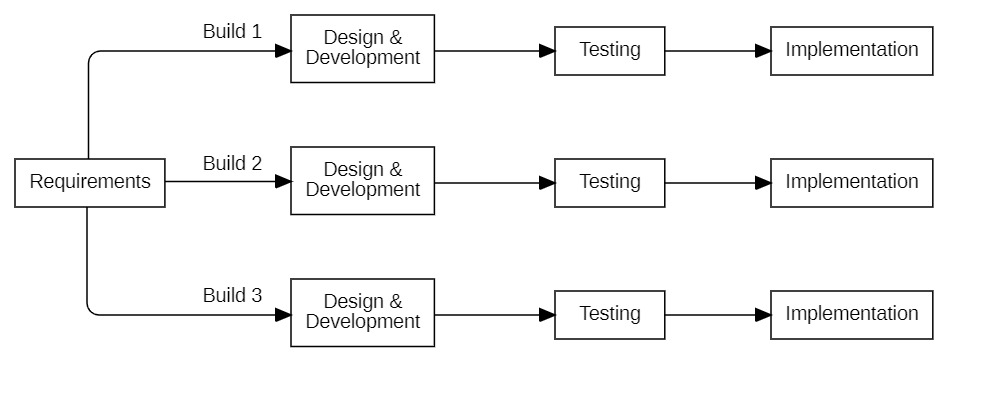
\includegraphics[scale=0.5]{images/incremental.jpg}
    \caption{Incremental Model}
    \label{fig:my_label}
\end{figure}
\section{Requirment Analysis}
\subsection{Functional Requirements}
\begin{itemize}
	\item The system should view the notices, results..
	\item The system should provide subscription feature for students of KEC only.
	\item The system should send result status email only to the subscribed accounts 
automatically after the publishment of result.
	\item The system should provide a feature to contact with admin of the website to 
report problems and error.

\end{itemize}
\subsection{Non-Functional requirements}

\begin{itemize}


	\item The system should be user friendly and easy to use.
	\item The system should be compatible and should run on almost all the device.
	\item The system should be reliable and responsive.
 
\end{itemize}

\chapter{Result and Discussion}

\section{Result}

We have completed the design and development of the project along with obtaining the 
desired output of the project. The project currently takes in the symbol number of the 
guest as well as subscribed users and shows the users the status of their current 
semester’s result. Along with this feature, the project also sends the status of the result 
automatically via email to the registered users, allows the user to view the notices 
published by IOE, allows the user to ask queries and report issues via “contact us” 
section and finally sends the activation email to the subscriber’s email to confirm the 
validity of the entered data. 

\section{Discussion}
IOE Result and Notice Viewer website is a website that takes in the symbol number of 
the guest as well as subscribed users and shows the users the status of their current 
semester’s result. Along with this feature, the project also sends the status of the result 
automatically via email to the registered users, allows the user to view the notices 
published by IOE, allows the user to ask queries and report issues via “contact us” 
section and finally sends the activation email to the subscriber’s email to confirm the 
validity of the entered data.
For the development of the website we used bootstrap, HTML, CSS, JavaScript to 
design the front end and of the website. The concept of web scraping was used to scrape 
IOE’s website for accessing the results and notices immediately after the publishment, 
OCR scan was also used to scan the symbol numbers of the passed student from the pdf 
file uploaded in the IOE’s website. These methods were implemented using python and 
Django along with MySQL as framework and database respectively.
Finally, after the completion of the project, the notices and results uploaded in the IOE’s
website up until the tenth page were scraped and stored in the database. And among the 
scraped notices and results, only results were selected and the OCR scan was used in 
the selected results to obtain the symbol numbers. After this, the symbol numbers along 
with the faculty, exam date, semester information were inserted into the database and 
19
using this data, the result status of the student was displayed to the guest users and the 
email about the status of the result was sent to the subscribers account automatically 
after the publishment of the result.

\section{Limitations}
\begin{itemize}
	\item Only the results that are published in BS Year 2079 can be viewed.
.
	\item After subscribing in case of any error form the user must contact the 
administrator as they cannot change it themselves.
	\item The user must fill up the form after every semester as the details will be changed.
	
	
\end{itemize}

\chapter{Conclusion and Future Enhancement}
\section{Conclusion}
In this project, we were able to design and build a website that helped the students of 
IOE to view the notices and result status after publishment. Also, only the students of 
Kantipur Engineering College could subscribe to the website to get the result status 
immediately via email after the publishment. The core of this system was designed 
using the web scraping and OCR. 

\section{Future Enhancement}
As our project still lacks in some sectors, further enhancements and improvements can
be made for the system to be more efficient and accurate, the following enhancements
can be done:

\begin{itemize}
	\item This project can be further extended into mobile applications so that a user can 
have one touch mobile experience.
	\item Implementation of login system for individual users for security and privacy.
	\item This project can be further extended to upload the mark sheet and store it in the 
database.
	

\end{itemize}

\newpage
%Reference
\renewcommand\bibname{REFERENCES} % Change heading to References
\bibliographystyle{IEEEtran} % to use IEEE Format for referencing
\addcontentsline{toc}{chapter}{References} % to add references in TOC
\bibliography{library} % specify the .bib file containing reference information 

\chapter*{ANNEX}
\addcontentsline{toc}{chapter}{Annex}
\begin{figure}[h]
    \centering
    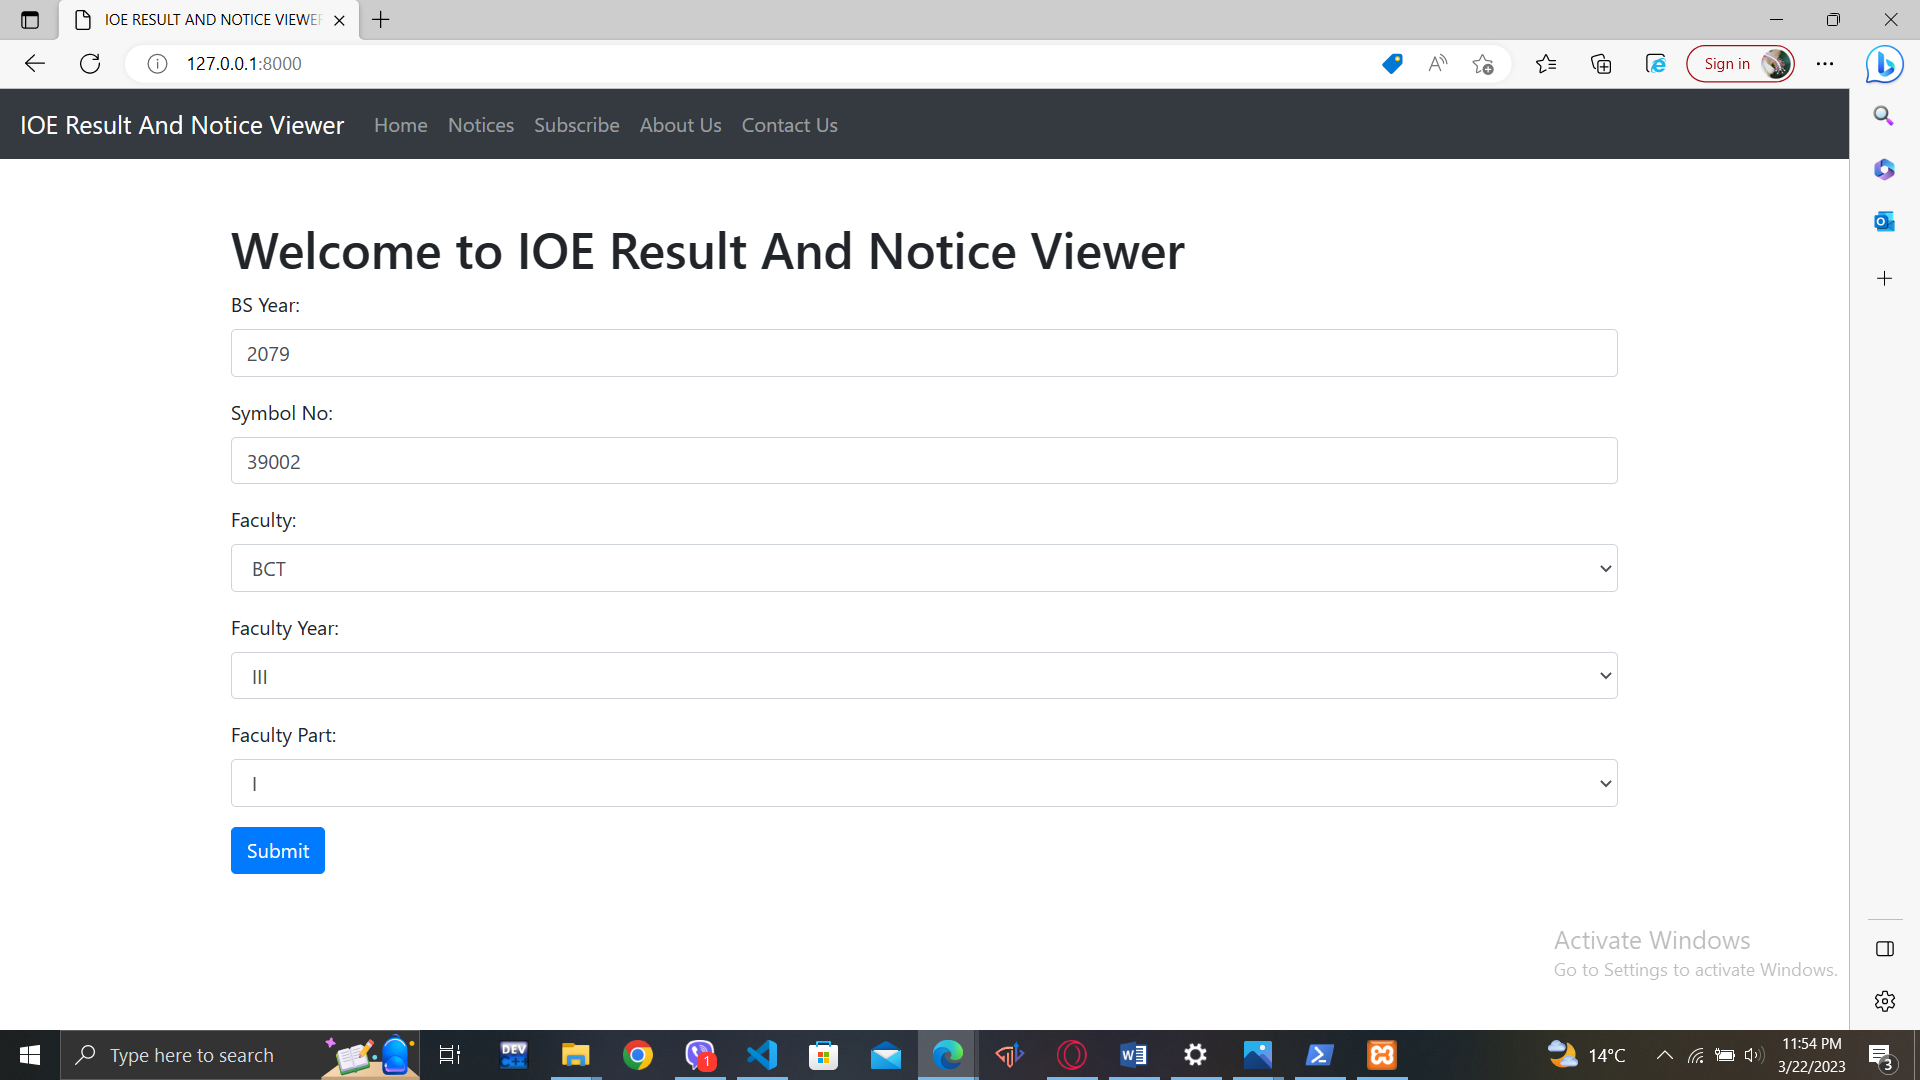
\includegraphics[scale=0.2]{pictures/1.png}
   % \caption{Gantt Chart}
   % \label{fig:my_label}
\end{figure}

\begin{figure}[h]
    \centering
    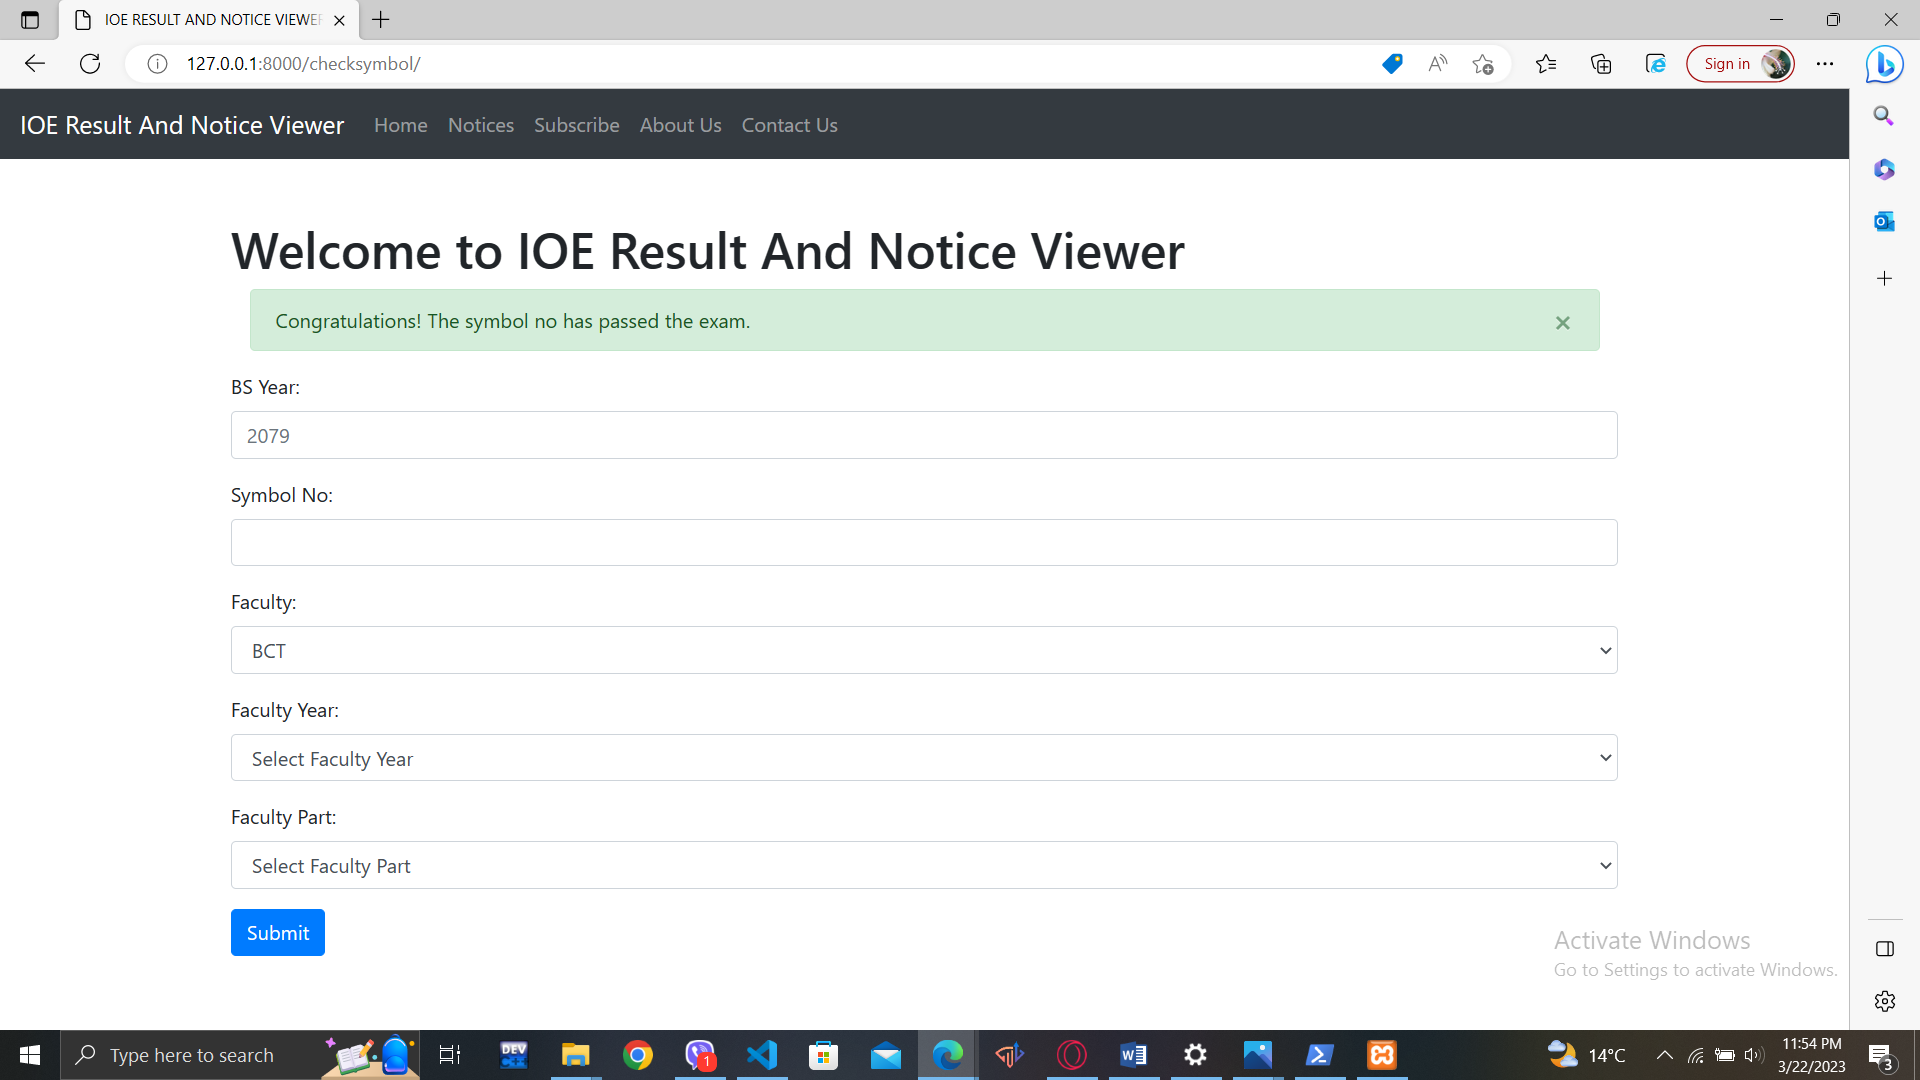
\includegraphics[scale=0.2]{pictures/2.png}
   % \caption{Gantt Chart}
   % \label{fig:my_label}
\end{figure}

\begin{figure}[h]
    \centering
    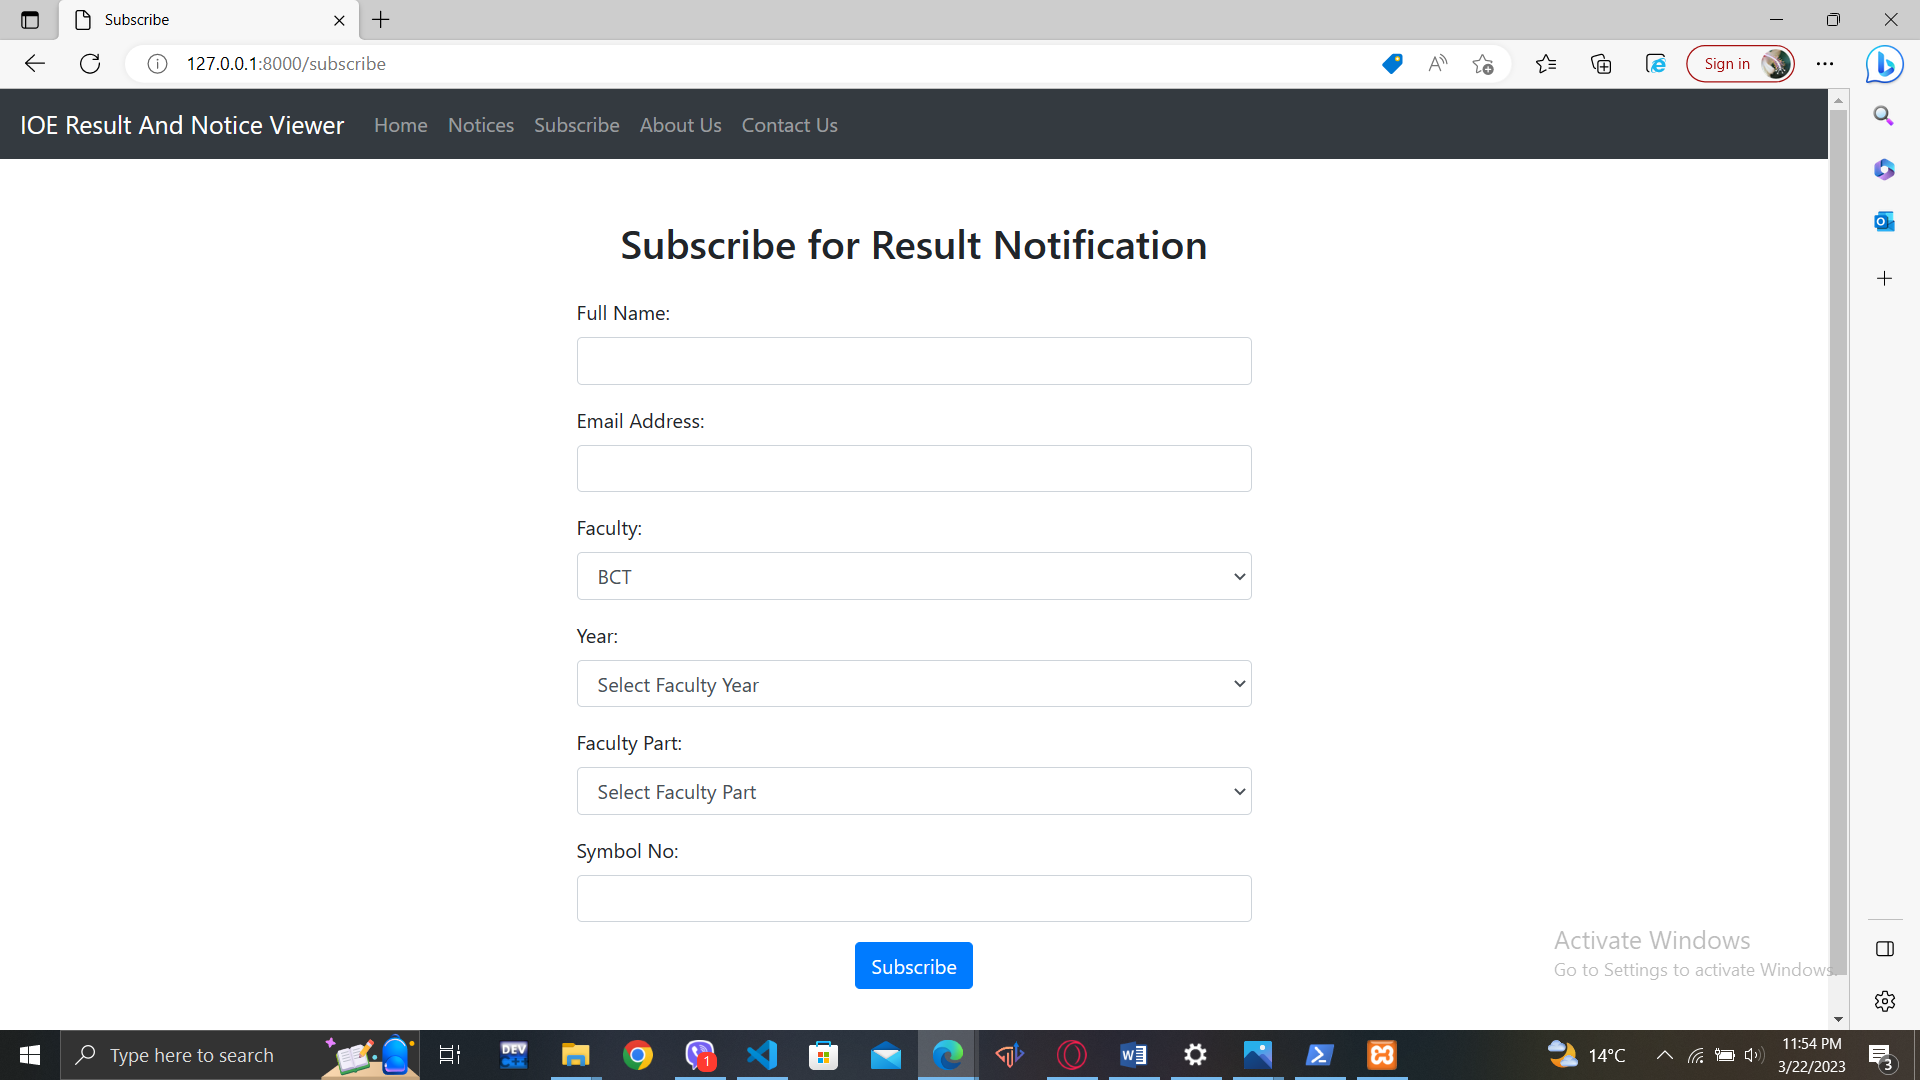
\includegraphics[scale=0.2]{pictures/3.png}
   % \caption{Gantt Chart}
   % \label{fig:my_label}
\end{figure}

\begin{figure}[h]
    \centering
    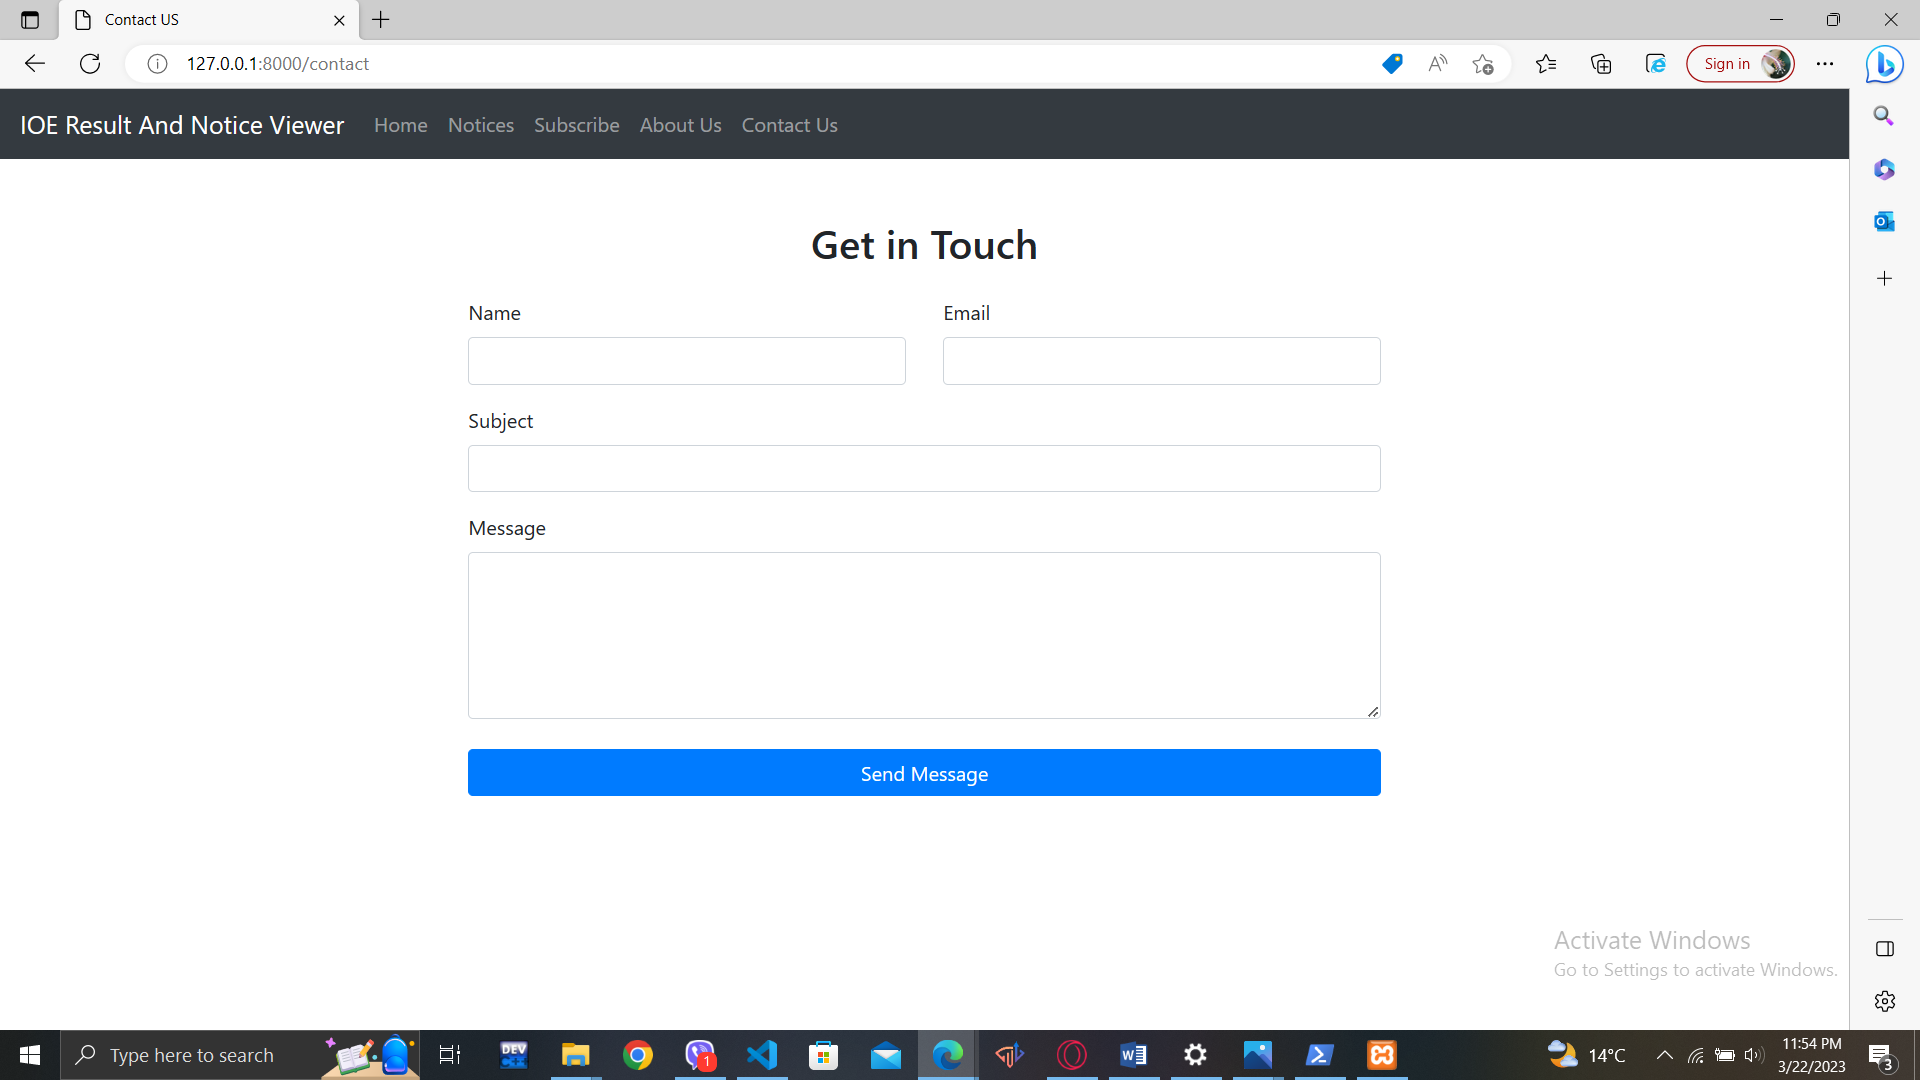
\includegraphics[scale=0.2]{pictures/4.png}
   % \caption{Gantt Chart}
   % \label{fig:my_label}
\end{figure}

\begin{figure}[h]
    \centering
    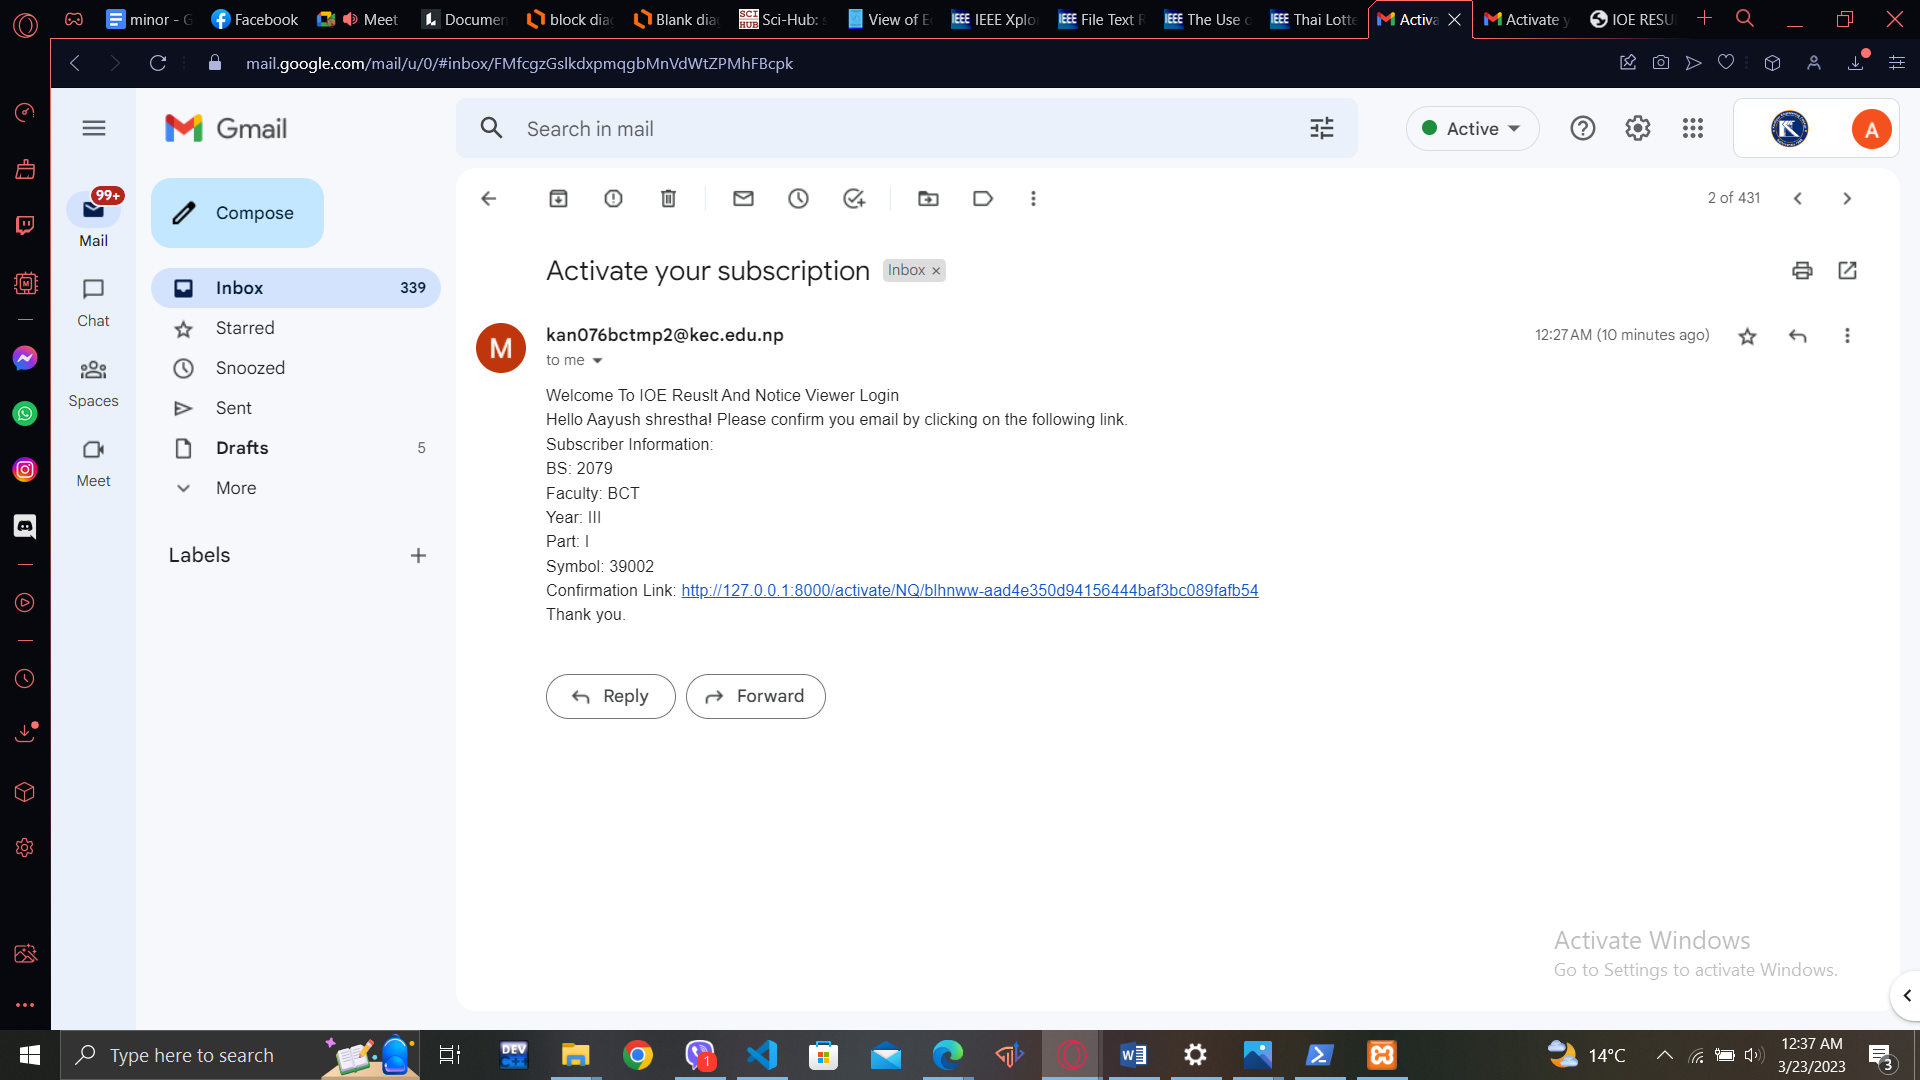
\includegraphics[scale=0.2]{pictures/5.png}
   % \caption{Gantt Chart}
   % \label{fig:my_label}
\end{figure}
\newpage
\begin{figure}[h]
    \centering
    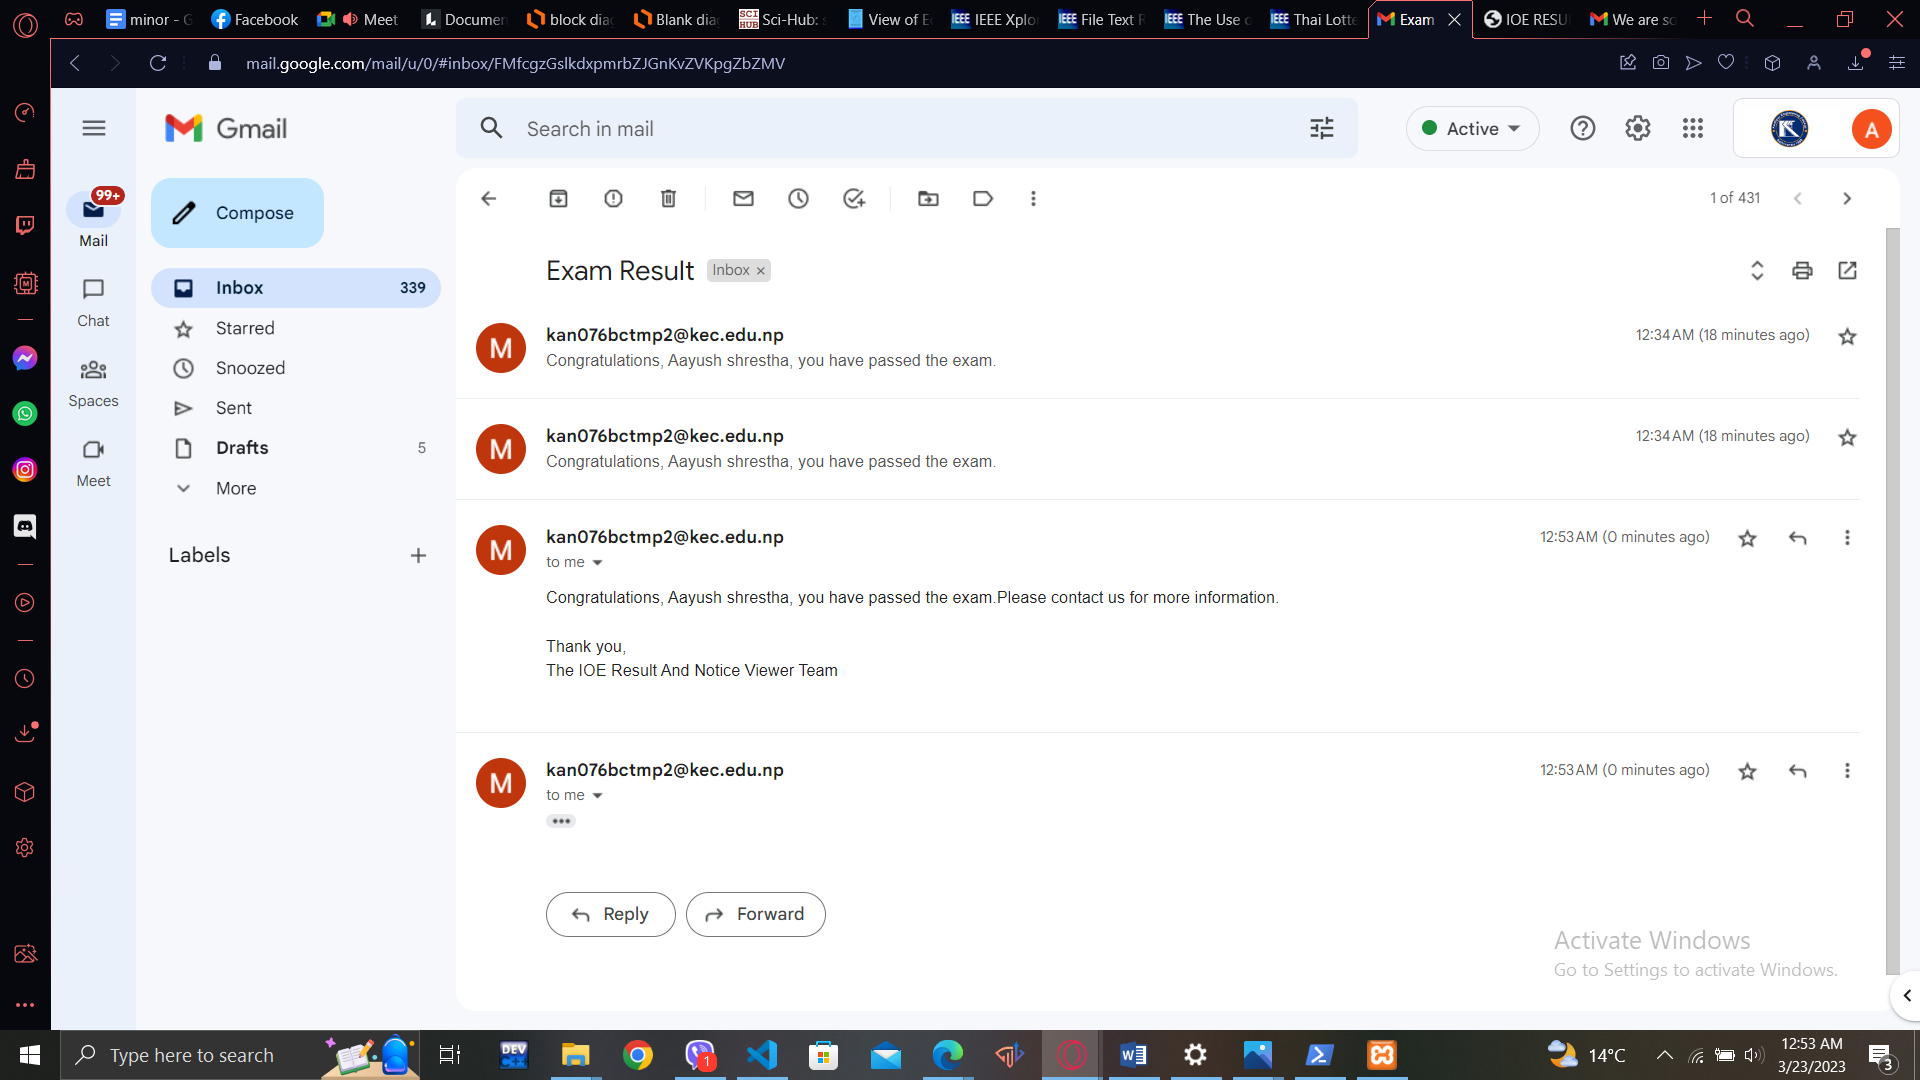
\includegraphics[scale=0.2]{pictures/6.png}
   % \caption{Gantt Chart}
   % \label{fig:my_label}
\end{figure}

\begin{figure}[h]
    \centering
    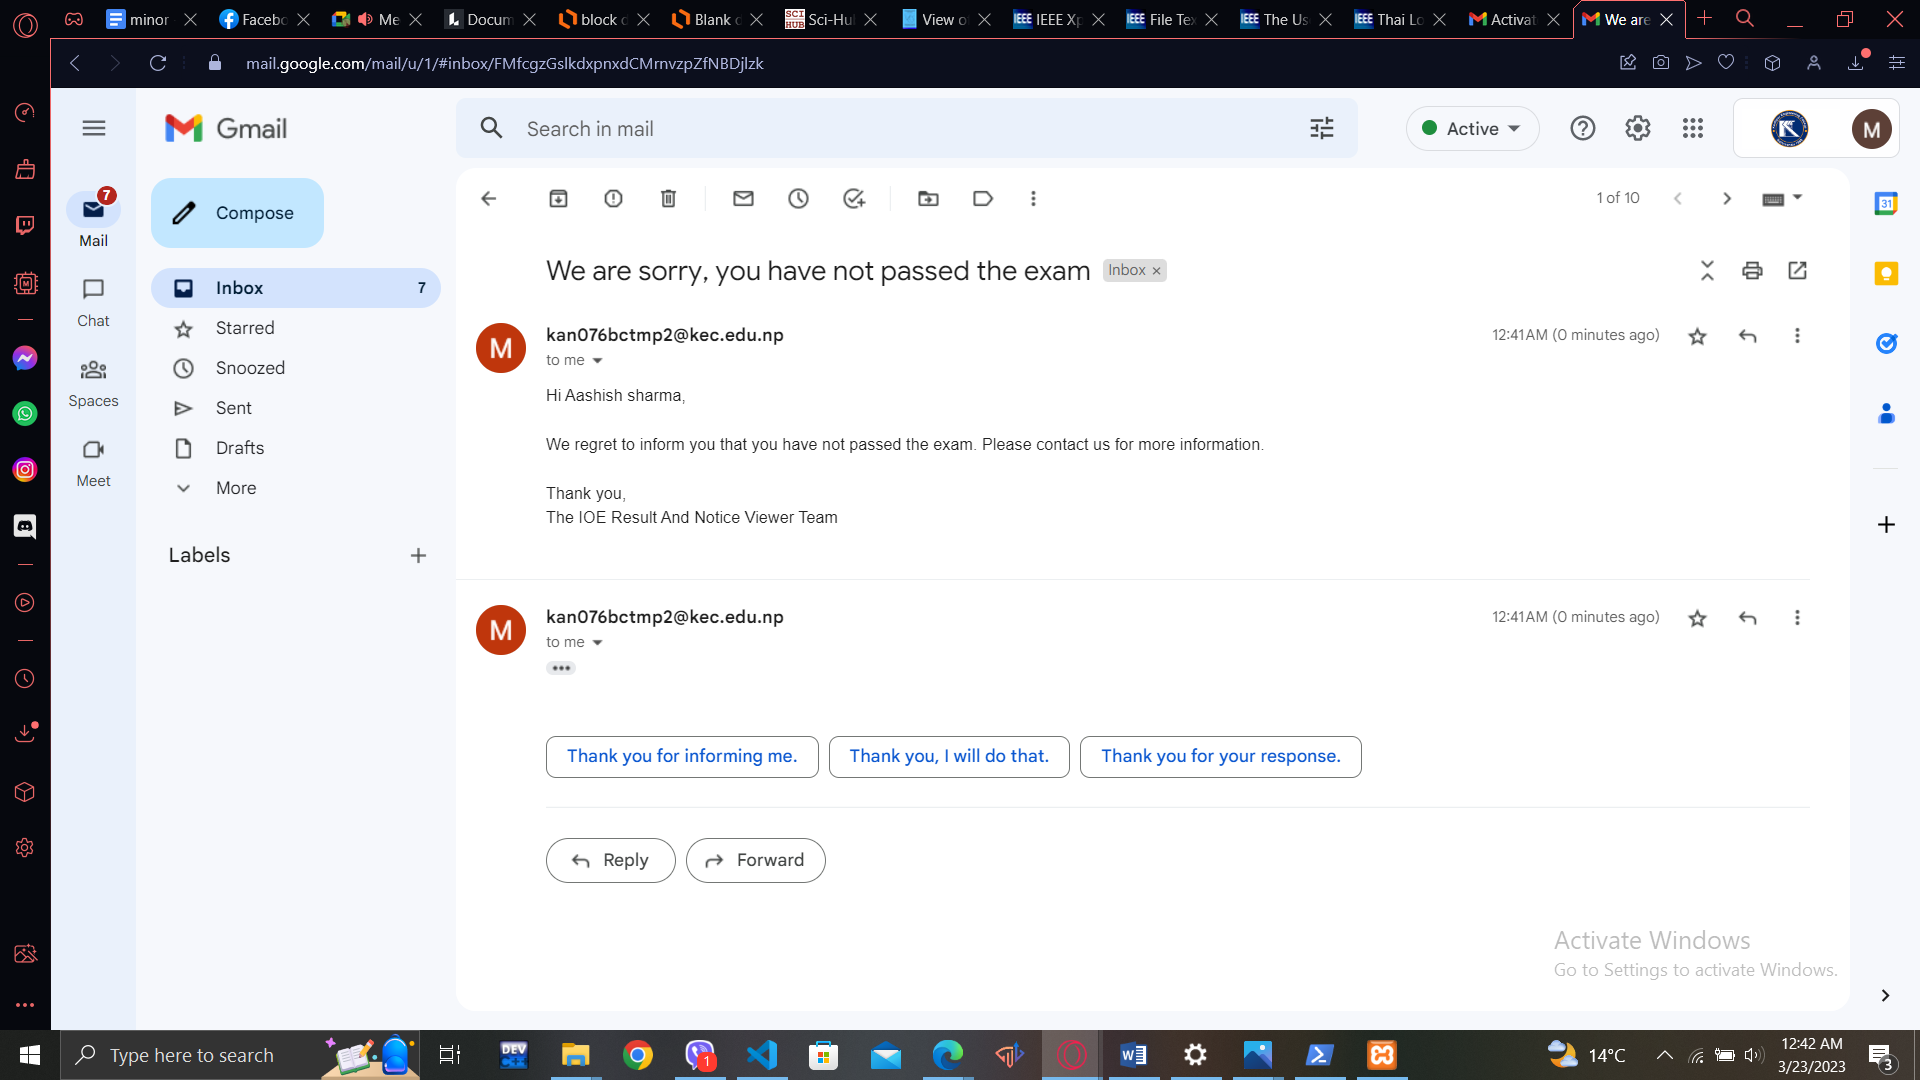
\includegraphics[scale=0.2]{pictures/7.png}
   % \caption{Gantt Chart}
   % \label{fig:my_label}
\end{figure}


\begin{figure}[h]
    \centering
    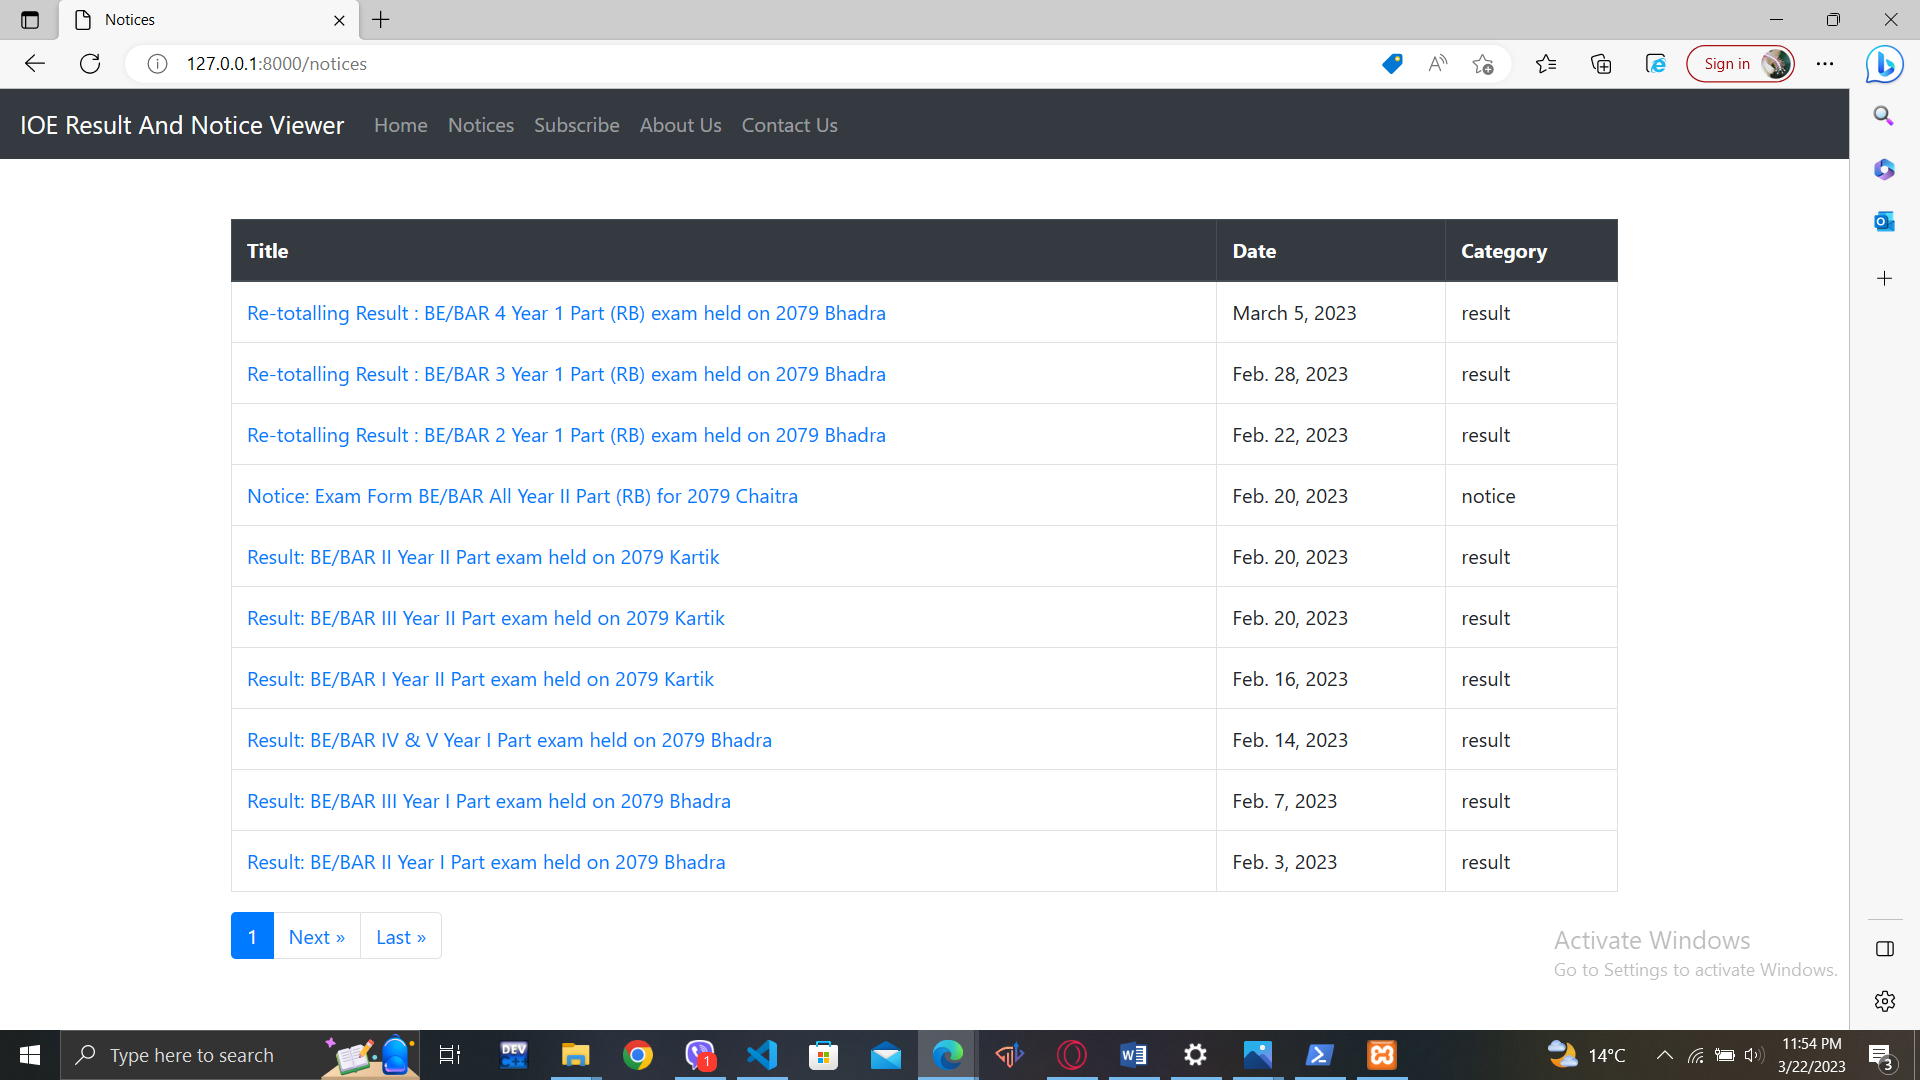
\includegraphics[scale=0.2]{pictures/8.png}
   % \caption{Gantt Chart}
   % \label{fig:my_label}
\end{figure}



%Comment this Chapter if you do not need to include Appendix.

%\addcontentsline{toc}{chapter}{Appendix}



	
\end{document}
